%%%  کلاس AUTthesis، نسخه آبان 1397
%%%   دانشگاه صنعتی امیرکبیر                 http://www.aut.ac.ir
%%%  تالار گفتگوی پارسی‌لاتک،       http://forum.parsilatex.com
%%%   آپدیت شده در آبان 95
%%%   پشتیبانی و راهنمایی          badali_farhad@yahoo.com
%%%
%%%   بازبینی و اصلاح شده در آبان ماه 1397
%%%  Tested via TeXstudio in TeXlive 2014-2018.
%%%

%-----------------------------------------------------------------------------------------------------
%        روش اجرا.: 2 بار F1 ، 2 بار  F11(به منظور تولید مراجع) ، دوبار Ctrl+Alt+I (به منظور تولید نمایه) و دو بار F1 -------> مشاهده Pdf
%%%%%%%%%%%%%%%%%%%%%%%%%%%%%%%%%%%%%%%%%%%%%%%%%%%%%%
%   TeXstudio as your IDE
%%  برای compile در TeXstudio تنها کافی است منوی Options->Configure TeXstudio را زده و در پنجره Configure TeXstudio در بخش Build گزینه Default Compiler را به XeLaTeX تغییر دهید. سند شما به راحتی compile خواهد شد.
%   F1 & F5 : Build & view
%   F6      : Compile
%   F7      : View
%   --------------
%%%%%%%%%%%%%%%%%%%%%%%%%%%%%%%%%%%%%%%%%%%%%%%%%%%%%%
%        اگر قصد نوشتن رساله دکتری را دارید، در خط زیر به جای msc،
%      کلمه phd را قرار دهید. کلیه تنظیمات لازم، به طور خودکار، اعمال می‌شود.
%%% !TEX TS-program = XeLaTeX
\documentclass[oneside,bsc,12pt]{AUTthesis}
%       فایل commands.tex را حتماً به دقت مطالعه کنید؛ چون دستورات مربوط به فراخوانی بسته زی‌پرشین 
%       و دیگر بسته‌ها و ... در این فایل قرار دارد و بهتر است که با نحوه استفاده از آنها آشنا شوید. توجه شود برای نسخه نهایی پایان‌نامه حتماً hyperref را 
%        غیرفعال کنید.



% در این فایل، دستورها و تنظیمات مورد نیاز، آورده شده است.
%-------------------------------------------------------------------------------------------------------------------
% در ورژن جدید زی‌پرشین برای تایپ متن‌های ریاضی، این سه بسته، حتماً باید فراخوانی شود.
\usepackage{amsthm,amssymb,amsmath,amsfonts}
% بسته‌ای برای تنطیم حاشیه‌های بالا، پایین، چپ و راست صفحه
\usepackage[top=30mm, bottom=30mm, left=25mm, right=30mm]{geometry}
% بسته‌‌ای برای ظاهر شدن شکل‌ها و تصاویر متن
\usepackage{graphicx}
\usepackage{color}
%بسته‌ای برای تنظیم فاصله عمودی خط‌های متن
\usepackage{setspace}
\usepackage{titletoc}
\usepackage{tocloft}
\usepackage{longtable}
\usepackage{tabularx}
	\newcolumntype{L}{>{\arraybackslash}X}
	%\newcolumntype{L}{>{\raggedright\arraybackslash}X}
\usepackage[utf8]{inputenc}
\usepackage[table]{xcolor}
\usepackage{float}
\definecolor{headerColor}{HTML}{d0d0d0}
%با فعال کردن بسته زیر فوت‌نوت‌ها در هر صفحه ریست می‌شوند. حالت پیش‌فرض آن ریست شدن در هر فصل است.
%\usepackage[perpage]{footmisc}
\usepackage{enumitem}
%\usepackage{titlesec}
% بسته‌ و دستوراتی برای ایجاد لینک‌های رنگی با امکان جهش
\usepackage[pagebackref=false,colorlinks,linkcolor=blue,citecolor=red]{hyperref}
\usepackage[nameinlink]{cleveref}%capitalize,,noabbrev
 \AtBeginDocument{%
    \crefname{equation}{برابری}{equations}%
    \crefname{chapter}{فصل}{chapters}%
    \crefname{section}{بخش}{sections}%
    \crefname{appendix}{پیوست}{appendices}%
    \crefname{enumi}{مورد}{items}%
    \crefname{footnote}{زیرنویس}{footnotes}%
    \crefname{figure}{شکل}{figures}%
    \crefname{table}{جدول}{tables}%
    \crefname{theorem}{قضیه}{theorems}%
    \crefname{lemma}{لم}{lemmas}%
    \crefname{corollary}{نتیجه}{corollaries}%
    \crefname{proposition}{گزاره}{propositions}%
    \crefname{definition}{تعریف}{definitions}%
    \crefname{result}{نتیجه}{results}%
    \crefname{example}{مثال}{examples}%
    \crefname{remark}{نکته}{remarks}%
    \crefname{note}{یادداشت}{notes}%
}
% چنانچه قصد پرینت گرفتن نوشته خود را دارید، خط بالا را غیرفعال و  از دستور زیر استفاده کنید چون در صورت استفاده از دستور زیر‌‌، 
% لینک‌ها به رنگ سیاه ظاهر خواهند شد که برای پرینت گرفتن، مناسب‌تر است
%\usepackage[pagebackref=false]{hyperref}
% بسته‌ لازم برای تنظیم سربرگ‌ها
\usepackage{fancyhdr}
% بسته‌ای برای ظاهر شدن «مراجع»  در فهرست مطالب
\usepackage[nottoc]{tocbibind}
% دستورات مربوط به ایجاد نمایه
\usepackage{makeidx,multicol,multirow}
\setlength{\columnsep}{1.5cm}

% \usepackage[round]{natbib}
% \bibliographystyle{plainnat}

%%%%%%%%%%%%%%%%%%%%%%%%%%
\usepackage{verbatim}
\makeindex
\usepackage{sectsty}

\usepackage{array}% for extended column definitions 
\newcommand{\PreserveBackslash}[1]{\let\temp=\\#1\let\\=\temp}
\newcolumntype{C}[1]{>{\PreserveBackslash\centering}p{#1}}
% فراخوانی بسته زی‌پرشین و تعریف قلم فارسی و انگلیسی
\usepackage{xepersian}%[extrafootnotefeatures]
\SepMark{-}
%حتماً از تک لایو 2014 استفاده کنید.
\settextfont[
    Scale=1.2,
    Path = ./fonts/, 
    BoldFont = BNaznnBd.ttf
]{BNazanin.ttf}

\setlatintextfont[
    Path = ./fonts/, 
    BoldFont = Georgia-Bold.ttf,
    ItalicFont = Georgia-Italic.ttf,
    BoldItalicFont = Georgia-Bold-Italic.ttf
]{Georgia.ttf}

\renewcommand{\labelitemi}{$\bullet$}
\renewcommand{\labelitemii}{$\circ$}
%%%%%%%%%%%%%%%%%%%%%%%%%%
% چنانچه می‌خواهید اعداد در فرمول‌ها، انگلیسی باشد، خط زیر را غیرفعال کنید.
%در غیر اینصورت حتماً فونت PGaramond را نصب کنید.
%\setdigitfont[Scale=1.1]{PGaramond}%%Yas
%%%%%%%%%%%%%%%%%%%%%%%%%%
% تعریف قلم‌های فارسی اضافی برای استفاده در بعضی از قسمت‌های متن
\defpersianfont\nastaliq[
Scale=2,
Path = ./fonts/,
]{IranNastaliq.ttf}

\defpersianfont\chapternumber[
    Scale=3,
    Path = ./fonts/, 
    BoldFont = BNaznnBd.ttf
]{BNazanin.ttf}
%\chapterfont{\centering}%
%%%%%%%%%%%%%%%%%%%%%%%%%%
% دستوری برای تغییر نام کلمه «اثبات» به «برهان»
\renewcommand\proofname{\textbf{برهان}}

% دستوری برای تغییر نام کلمه «کتاب‌نامه» به «منابع و مراجع«
\renewcommand{\bibname}{منابع و مراجع}


% Headings for every page of ToC, LoF and Lot
\setlength{\cftbeforetoctitleskip}{-1.2em}
\setlength{\cftbeforelottitleskip}{-1.2em}
\setlength{\cftbeforeloftitleskip}{-1.2em}
\setlength{\cftaftertoctitleskip}{-1em}
\setlength{\cftafterlottitleskip}{-1em}
\setlength{\cftafterloftitleskip}{-1em}
%%\makeatletter
%%%%\renewcommand{\l@chapter}{\@dottedtocline{1}{1em\bfseries}{1em}}
%%%%\renewcommand{\l@section}{\@dottedtocline{2}{2em}{2em}}
%%%%\renewcommand{\l@subsection}{\@dottedtocline{3}{3em}{3em}}
%%%%\renewcommand{\l@subsubsection}{\@dottedtocline{4}{4em}{4em}}
%%%%\makeatother


\newcommand\tocheading{\par عنوان\hfill صفحه \par}
\newcommand\lofheading{\hspace*{.5cm}\figurename\hfill صفحه \par}
\newcommand\lotheading{\hspace*{.5cm}\tablename\hfill صفحه \par}

\renewcommand{\cftchapleader}{\cftdotfill{\cftdotsep}}
\renewcommand{\cfttoctitlefont}{\hspace*{\fill}\LARGE\bfseries}%\Large
\renewcommand{\cftaftertoctitle}{\hspace*{\fill}}
\renewcommand{\cftlottitlefont}{\hspace*{\fill}\LARGE\bfseries}%\Large
\renewcommand{\cftafterlottitle}{\hspace*{\fill}}
\renewcommand{\cftloftitlefont}{\hspace*{\fill}\LARGE\bfseries}
\renewcommand{\cftafterloftitle}{\hspace*{\fill}}

%%%%%%%%%%%%%%%%%%%%%%%%%%
% تعریف و نحوه ظاهر شدن عنوان قضیه‌ها، تعریف‌ها، مثال‌ها و ...
%برای شماره گذاری سه تایی قضیه‌ها
\theoremstyle{definition}
\newtheorem{definition}{تعریف}[section]
\newtheorem{remark}[definition]{نکته}
\newtheorem{note}[definition]{یادداشت}
\newtheorem{example}[definition]{نمونه}
\newtheorem{question}[definition]{سوال}
\newtheorem{remember}[definition]{یاداوری}
\theoremstyle{theorem}
\newtheorem{theorem}[definition]{قضیه}
\newtheorem{lemma}[definition]{لم}
\newtheorem{proposition}[definition]{گزاره}
\newtheorem{corollary}[definition]{نتیجه}
%%%%%%%%%%%%%%%%%%%%%%%%
%%%%%%%%%%%%%%%%%%%
%%% برای شماره گذاری چهارتایی قضیه‌ها و ...
%%\newtheorem{definition1}[subsubsection]{تعریف}
%%\newtheorem{theorem1}[subsubsection]{قضیه}
%%\newtheorem{lemma1}[subsubsection]{لم}
%%\newtheorem{proposition1}[subsubsection]{گزاره}
%%\newtheorem{corollary1}[subsubsection]{نتیجه}
%%\newtheorem{remark1}[subsubsection]{نکته}
%%\newtheorem{example1}[subsubsection]{مثال}
%%\newtheorem{question1}[subsubsection]{سوال}

%%%%%%%%%%%%%%%%%%%%%%%%%%%%

% دستورهایی برای سفارشی کردن صفحات اول فصل‌ها
\makeatletter
\newcommand\mycustomraggedright{%
 \if@RTL\raggedleft%
 \else\raggedright%
 \fi}
\def\@makechapterhead#1{%
\thispagestyle{style1}
\vspace*{20\p@}%
{\parindent \z@ \mycustomraggedright
\ifnum \c@secnumdepth >\m@ne
\if@mainmatter

\bfseries{\Huge \@chapapp}\small\space {\chapternumber\thechapter}
\par\nobreak
\vskip 0\p@
\fi
\fi
\interlinepenalty\@M 
\Huge \bfseries #1\par\nobreak
\vskip 120\p@

}

%\thispagestyle{empty}
\newpage}
\bidi@patchcmd{\@makechapterhead}{\thechapter}{\tartibi{chapter}}{}{}
\bidi@patchcmd{\chaptermark}{\thechapter}{\tartibi{chapter}}{}{}
\makeatother

\pagestyle{fancy}
\renewcommand{\chaptermark}[1]{\markboth{\chaptername~\tartibi{chapter}: #1}{}}

\fancypagestyle{style1}{
\fancyhf{} 
\fancyfoot[c]{\thepage}
\fancyhead[R]{\leftmark}%
\renewcommand{\headrulewidth}{1.2pt}
}


\fancypagestyle{style2}{
\fancyhf{}
\fancyhead[R]{چکیده}
\fancyfoot[C]{\thepage{}}
\renewcommand{\headrulewidth}{1.2pt}
}

\fancypagestyle{style3}{%
  \fancyhf{}%
  \fancyhead[R]{فهرست نمادها}
  \fancyfoot[C]{\thepage}%
  \renewcommand{\headrulewidth}{1.2pt}%
}

\fancypagestyle{style4}{%
  \fancyhf{}%
  \fancyhead[R]{فهرست جداول}
  \fancyfoot[C]{\thepage}%
  \renewcommand{\headrulewidth}{1.2pt}%
}

\fancypagestyle{style5}{%
  \fancyhf{}%
  \fancyhead[R]{فهرست اشکال}
  \fancyfoot[C]{\thepage}%
  \renewcommand{\headrulewidth}{1.2pt}%
}

\fancypagestyle{style6}{%
  \fancyhf{}%
  \fancyhead[R]{فهرست مطالب}
  \fancyfoot[C]{\thepage}%
  \renewcommand{\headrulewidth}{1.2pt}%
}

\fancypagestyle{style7}{%
  \fancyhf{}%
  \fancyhead[R]{نمایه}
  \fancyfoot[C]{\thepage}%
  \renewcommand{\headrulewidth}{1.2pt}%
}

\fancypagestyle{style8}{%
  \fancyhf{}%
  \fancyhead[R]{منابع و مراجع}
  \fancyfoot[C]{\thepage}%
  \renewcommand{\headrulewidth}{1.2pt}%
}
\fancypagestyle{style9}{%
  \fancyhf{}%
  \fancyhead[R]{واژه‌نامه‌ی فارسی به انگلیسی}
  \fancyfoot[C]{\thepage}%
  \renewcommand{\headrulewidth}{1.2pt}%
}
%

%دستور حذف نام لیست تصاویر و لیست جداول از فهرست مطالب
\newcommand*{\BeginNoToc}{%
  \addtocontents{toc}{%
    \edef\protect\SavedTocDepth{\protect\the\protect\value{tocdepth}}%
  }%
  \addtocontents{toc}{%
    \protect\setcounter{tocdepth}{-10}%
  }%
}
\newcommand*{\EndNoToc}{%
  \addtocontents{toc}{%
    \protect\setcounter{tocdepth}{\protect\SavedTocDepth}%
  }%
}
\newcounter{savepage}
\renewcommand{\listfigurename}{فهرست اشکال}
\renewcommand{\listtablename}{فهرست جداول}
\usepackage{booktabs}% http://ctan.org/pkg/booktabs
\newcommand{\tabitem}{~~\llap{\textbullet}~~}
%\renewcommand\cftsecleader{\cftdotfill{\cftdotsep}}
%%%%%%%%%%%%%%%%%%%%%%%%%%%%%
%%%%%%%%%%%%%%%%%%%%%%%%%%%%
\begin{document}
\baselineskip=.75cm
\linespread{1.75}
%% -!TEX root = AUTthesis.tex
% در این فایل، عنوان پایان‌نامه، مشخصات خود، متن تقدیمی‌، ستایش، سپاس‌گزاری و چکیده پایان‌نامه را به فارسی، وارد کنید.
% توجه داشته باشید که جدول حاوی مشخصات پروژه/پایان‌نامه/رساله و همچنین، مشخصات داخل آن، به طور خودکار، درج می‌شود.
%%%%%%%%%%%%%%%%%%%%%%%%%%%%%%%%%%%%
% دانشکده، آموزشکده و یا پژوهشکده  خود را وارد کنید

\faculty{دانشکده مهندسی کامپیوتر}
% گرایش و گروه آموزشی خود را وارد کنید
\department{}
% عنوان پایان‌نامه را وارد کنید
\fatitle{رابط ارتباطي تحت وب خدمات زيرساخت بعنوان خدمت \lr{VCloud}
\\[.75 cm]
}
% نام استاد(ان) راهنما را وارد کنید
\firstsupervisor{دکتر محمود ممتازپور}
%\secondsupervisor{استاد راهنمای دوم}
% نام استاد(دان) مشاور را وارد کنید. چنانچه استاد مشاور ندارید، دستور پایین را غیرفعال کنید.
% \firstadvisor{دکتر مهدی همایون‌پور}
%\secondadvisor{استاد مشاور دوم}
% نام نویسنده را وارد کنید
\name{سیدمحمد}
% نام خانوادگی نویسنده را وارد کنید
\surname{فاطمی}
%%%%%%%%%%%%%%%%%%%%%%%%%%%%%%%%%%
\thesisdate{اسفند ۱۴۰۱}

% چکیده پایان‌نامه را وارد کنید
\fa-abstract{
امروزه الگوی مصرف منابع محاسباتی و شبکه‌ای بسیار به الگوی رایانش ابری نزدیک شده‌است. با این وجود ارائه دهندگان خدمات زیرساخت در داخل کشور همچنان فاصله زیادی تا ارائه خدمات منطبق بر الگوی رایانش ابری دارند. یکی از خدمات معروف مورد نیاز کاربران، نیاز به زیرساخت به عنوان خدمت است. چالش پیاده‌سازی این خدمت، پیاده‌سازی زیرساخت و درگاه‌های مورد نیاز جهت تحویل خدمات به کاربر است. در مورد مسئله اول، راه‌حل‌های متن‌باز و صنعتی متعددی ارائه شده‌اند. ایراد استفاده مستقیم از این راه‌حل‌های بدون نیاز به تغییر و پیاده‌سازی درگاه ارتباطی خصوصی، عدم امکان شخصی‌سازی امکانات و نحوه ارائه خدمات است. به علت متفاوت بودن الگو‌های ارائه‌ی خدمت و مدیریت کاربران، این ابزار‌ها، پیاده‌سازی این قسمت از سامانه‌ را برعهده‌ی ‌کاربر استفاده کننده قرار داده‌اند. در این پروژه به بررسی نیازمندی‌های یک سامانه‌ی ارائه‌ی خدمات زیرساخت به عنوان خدمت پرداخته شده و با بررسی و مشخص کردن نیازمندی‌ها و فناوری‌ها، یک رابط برنامه‌نویسی تحت وب برای خدمات مطرح شده بر روی زیرساخت \lr{VMWare Cloud Director} ارائه شده‌است. در مراحل مختلف طراحی، تصمیمات و گزینه‌های مختلف مطرح شده و دلیل تصمیم گیری‌ها و انتخاب فناوری شرح داده شده‌است. پس از پیاده‌سازی، با طرح و اجرای ارزیابی‌های مختلف بر روی این راه‌حل، از صحت عملکرد آن در سناریو‌های واقعی اطمینان حاصل پیدا شده‌است. در انتها با بررسی کلیت سامانه، نقاط بهبود و جایگاه‌های قابل توسعه در پروژه شرح داده‌شده که بتوان در جهت‌های مختلف این پروژه را توسعه داد و خدمات جامع‌تری را پوشش داد.
}
%توجه: ‌در اعداد اعشاری قسمت صحیح و اعشار جا به جا باید نوشته شوند تا در متن به طور صحیح نمایش داده شوند. به عنوان مثال در متن بالا عدد ۲۹.۰۷ را جا به جا وارد کرده تا در متن به طور صحیح نمایش داده شود. 

% کلمات کلیدی پایان‌نامه را وارد کنید
\keywords{رایانش ابری، زیرساخت به عنوان خدمت، رابط برنامه‌نویسی تحت وب، معماری میکروسرویس}


\AUTtitle
%%%%%%%%%%%%%%%%%%%%%%%%%%%%%%%%%%
\vspace*{7cm}
\thispagestyle{empty}
\begin{center}

\includegraphics[height=5cm,width=12cm]{besm}
\end{center}
% تاییدیه دفاع
\newpage
\thispagestyle{empty}
%\fontsize{18pt}{19pt}\selectfont

\section*{صفحه فرم ارزیابی و تصویب پایان نامه- فرم تأیید اعضاء كميته دفاع}

\fontsize{12pt}{14pt}\selectfont
%\renewcommand{\baselinestretch}{1.5}
\vspace*{1cm}
   در این صفحه فرم دفاع یا تایید و تصویب پایان نامه موسوم به فرم کمیته دفاع- موجود در پرونده آموزشی- را قرار دهید.
\vspace*{1cm}


\subsection*{نکات مهم:}
 
\begin{itemize}
\item
	نگارش پایان نامه/رساله باید به
	{\color{red}
		زبان فارسی
	}
	و بر اساس آخرین نسخه دستورالعمل و راهنمای تدوین پایان نامه‌های دانشگاه صنعتی امیرکبیر باشد.(دستورالعمل و راهنمای حاضر)
\item رنگ جلد پایان نامه/رساله چاپي كارشناسي، كارشناسي ارشد و دكترا  بايد به ترتيب مشكي، طوسي و سفيد رنگ باشد.  
\item چاپ و صحافی پایان نامه/رساله بصورت
{\color{red}
	پشت و رو(دورو)
}
بلامانع است و انجام آن توصيه مي شود. 
\end{itemize}
%%%%%%%%%%%%%%%%%%%%%%%%%%%%%%%%%%%%%%%%%%%%%%%%%%%%%%%%%%%%%%%%%%%%%%%%%%%%%%%%%%%%%%%%%%%%%%%%%%
%%%%%%%%%%%%%%%%%%%%%%%%%%%%%%%%%%%%%%%%%%%%%%%%%%%%%%%%%%%%%%%%%%%%%%%%%%%%%%%%%%%%%%%%%%%%%%%%%%
\newpage
\thispagestyle{empty}
\begin{picture}(50,50)
  \put(17,0){
\includegraphics[scale=1.1]{fa-logo}}
  \put(4.5,-13){\footnotesize{دانشگاه صنعتی امیرکبیر}}
  \put(10.5,-27){\footnotesize{(پلی‌تکنیک تهران)}}
  \put(170,30){\bf{به نام خدا}}
  \put(140,-5){\Large\bf{تعهدنامه اصالت اثر}}
  \put(310,0){تاریخ: \datethesis}
\end{picture}

\vspace*{2.5cm}

اينجانب {\bf{\fname\lname}} متعهد می‌شوم که مطالب مندرج در این پایان‌نامه حاصل کار پژوهشی اینجانب تحت نظارت و راهنمایی اساتید دانشگاه صنعتی امیرکبیر بوده و به دستاوردهای دیگران که در این پژوهش از آنها استفاده شده است مطابق مقررات و روال متعارف ارجاع و در فهرست منابع و مآخذ ذکر گردیده است. این پایان‌نامه قبلاً برای احراز هیچ مدرک هم‌سطح یا بالاتر ارائه نگردیده است.

در صورت اثبات تخلف در هر زمان، مدرک تحصیلی صادر شده توسط دانشگاه از درجه اعتبار ساقط بوده و دانشگاه حق پیگیری قانونی خواهد داشت.


کلیه نتایج و حقوق حاصل از این پایان‌نامه متعلق به دانشگاه صنعتی امیرکبیر است. هرگونه استفاده از نتایج علمی و عملی، واگذاری اطلاعات به دیگران یا چاپ و تکثیر، نسخه‌برداری، ترجمه و اقتباس از این پایان نامه بدون موافقت کتبی دانشگاه صنعتی امیرکبیر ممنوع است. 
نقل مطالب با ذکر مآخذ بلامانع است.\\
\vspace{2.5cm}


{\centerline {\bf{\fname\lname}}}
\vspace*{.2cm}
{\centerline{امضا}}
%%%%%%%%%%%%%%%%%%%%%%%%%%%%%%%%%
% چنانچه مایل به چاپ صفحات «تقدیم»، «نیایش» و «سپاس‌گزاری» در خروجی نیستید، خط‌های زیر را با گذاشتن ٪  در ابتدای آنها غیرفعال کنید.
% پایان‌نامه خود را تقدیم کنید
% نیایش خود را در فایل زیر بنویسید.
\begin{acknowledgementpage}

\vspace{1.5cm}

{\nastaliq
{
تقدیم به \\
آن‌که جز به فضلش امیدی نیست...\\
}}\end{acknowledgementpage}
\newpage
% سپاسگزاری را در فایل زیر بنویسید.
%%%%%%%%%%%%%%%%%%%%%%%%%%%%%%%%%%%%
\newpage\thispagestyle{empty}
% سپاس‌گزاری
{\nastaliq
سپاس‌گزاری
}
\\[2cm]

 از پدر و مادرم که همواره در مواجهه با سختی‌های این دنیا دلسوزانه همراهم بوده‌اند؛\\
 از استاد بزرگوارم جناب آقای دکتر محمود ممتازپور که با حسن خلق و گشاده‌رویی، رهنمودهای شبانه‌روزی خود را از من دریغ نکرده‌اند؛\\
و از سایر عزیزانی که در کنارشان این نتیحه حاصل آمد کمال تشکر و قدردانی را دارم.

\signature








%%%%%%%%%%%%%%%%%%%%%%%%%%%%%%%%%%%%%%%%%
%%%%%%%%%%%%%%%%%%%%%%%%%%%%%%%%%کدهای زیر را تغییر ندهید.
\newpage\clearpage

\pagestyle{style2}

\vspace*{-1cm}
\section*{\centering چکیده}
% \addcontentsline{toc}{chapter}{چکیده}
\vspace*{.5cm}
\ffa-abstract
\vspace*{2cm}


{\noindent\large\textbf{واژه‌های کلیدی:}}\par
\vspace*{.5cm}
\fkeywords
% دستور زیر برای شماره گذاری صفحات قبل از فصل اول با حروف ابجد است.
\pagenumbering{alph}
%-----------------------------------------------------------------------------
% فایل زیر دستورات مربوط به نمایش صفحات فهرست مطالب- فهرست اشکال و جداول است.
%{\pagestyle{style2}
%\tableofcontents}\newpage
%
%\listoffigures
\cleardoublepage
\pagestyle{style6}
\tableofcontents
\pagestyle{style6}
\cleardoublepage
%اگر لیست تصاویر و لیست جداول ندارید ، کدهای زیر را با گذاشتن % در ابتدای آنها، غیرفعال کنید.
\BeginNoToc
%============
\addtocontents{lof}{\lofheading}% add heading to the first page in LoF
\pagestyle{style5}
\listoffigures
\thispagestyle{style5}
\cleardoublepage
%============
\addtocontents{lot}{\lotheading}% add heading to the first page in LoT
\thispagestyle{style4}
\listoftables
\thispagestyle{style4}
%============
%\cleardoublepage
%
\cleardoublepage
\setcounter{savepage}{\arabic{page}}
\mainmatter
\addtocontents{toc}{\tocheading}% add heading to the first page in ToC, after frontmatter entries
\EndNoToc
% در صورت تمایل می‌توانید با فعال کردن دستور بالا، لیست تصاویر را به  پایان‌نامه خود اضافه کنید.
%-------------------------------------------------------------------------symbols(فهرست نمادها)
% وجود لیست نمادها الزامیست.(لطفاً نمادهای خود را جایگذین نمادهای پیش‌فرض کنید.)
%%%%%%%%%%%%%
%\addcontentsline{toc}{chapter}{فهریست نمادها}
\setcounter{page}{\thesavepage}
\vspace*{1cm}
\pagestyle{empty}
\thispagestyle{empty}
\newpage

\pagenumbering{arabic}
\pagestyle{style1}
%--------------------------------------------------------------------------chapters(فصل ها)
\chapter{مقدمه}
\section{مقدمه}
رایانش ابری\LTRfootnote{Cloud Computing} یکی از حوزه‌های در حال تحول کامپیوتر است که به یک جنبه‌ی حیاتی از فناوری و مشاغل مدرن تبدیل شده است. این الگو همچون انقلابی، شیوه‌ی ارائه و مصرف منابع محاسباتی را متحول کرده است و فرصت‌های جدیدی را برای سازمان‌ها فراهم کرده تا کارایی و رقابت خود را بهبود بخشند. یکی از پایه‌ای‌ترین و رایج‌ترین شکل‌های رایانش ابری، زیرساخت به عنوان خدمت (\lr{IaaS})\LTRfootnote{Infrastructure As A Service} است که منابع محاسباتی مجازی مانند فضای ذخیره‌سازی، قدرت پردازش و پهنای باند را از طریق اینترنت در اختیار کاربران قرار می‌دهد\cite{Mell_2011}.

\begin{figure}[h]
	\vspace{1cm}
	\centering
	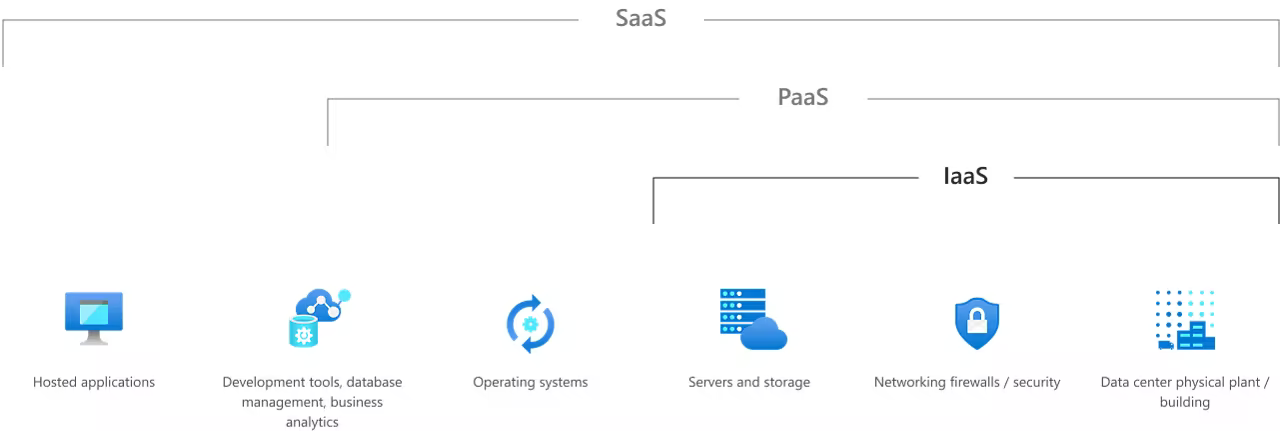
\includegraphics[scale=0.35]{figures/cloud_computing_models.png}
	\caption{انواع مدل‌های رایانش ابری\cite{microsoft_cc_models}}
	\label{fig:cc_models}
\end{figure}

این الگو را از دو دیدگاه می‌توان بررسی کرد. دیدگاه اول مختص کاربران مصرف‌کننده است که برای استفاده و مصرف منابع دیگر دغدغه‌ای نسبت به زیرساخت استفاده شده برای ارائه‌ی خدمات ندارند. دیدگاه دوم مربوط به ارائه دهندگان این خدمت است. از این دیدگاه، توسعه یک سکو\LTRfootnote{Platform} کارآمد و قابل اعتماد که بتواند مشتریان را جذب و حفظ کند، بسیار مهم است. از این رو، شرکت‌ها و توسعه‌دهندگان سراسر دنیا همواره سعی در توسعه و فراهم‌کردن ابزارها با این هدف دارند. یکی از معروف‌ترین این شرکت‌ها، شرکت \lr{VMWare} است که برنامه‌های فراوانی برای فراهم کردن زیرساخت ارائه‌ی خدمات ابری توسعه داده است. چالش بعدی ارائه‌دهندگان، فراهم کردن و طراحی یک رابط برنامه‌نویسی (\lr{API})\LTRfootnote{Application Programming Interface} است که بتواند با مشتریان و ارائه دهنده زیرساخ\LTRfootnote{Infrastructure Provider} تعامل داشته‌باشد و آن‌ها را قادر سازد منابع مجازی خود را مدیریت کنند.
\section{تعریف مسئله}
در این پروژه قصد داریم که خدمات جامع یک ارائه‌دهنده‌ی زیرساخت به عنوان خدمت را که بر بستر ابزار \LTRfootnote{https://vmware.com/products/cloud-director.html}\lr{VMWare Cloud Director} فراهم شده است را توسط یک رابط برنامه‌نویسی به کاربران ارائه دهیم. برای این هدف، باید خدمات کاربردی، مدیریتی، نظارتی و امنیتی را در یک لایه‌ی جدا تعریف کنیم و این لایه از برنامه‌ی خود را با ابزار زیرساختی در تعامل نگه داریم. 
\section{راه حل پیشنهادی}
برای توسعه این محصول، بایستی در ابتدا با بررسی نیازمندی‌ها و محدودیت‌های زیرساخت و کاربران، اقدام به طراحی کلی سامانه کرد. با توجه به گسترده بودن این نیازمندی‌ها و توسعه‌پذیری جداگانه آن‌ها، باید طراحی کلی این سامانه به صورت پیمانه‌ای\LTRfootnote{Modular} و با کمترین وابستگی میان واحد‌ها باشد. در این گزارش، ابتدا به طراحی و شرح قسمت‌های مختلف سامانه می‌پردازیم و سپس جزئیات فنی هر قسمت و تعامل قسمت‌ها را بررسی می‌کنیم.


هدف ما، پیاده‌سازی یک سامانه‌ی کاربردی کامل است که با استفاده از رابط برنامه‌نویسی تحت وب، بتوانیم خدمات را از آن دریافت کنیم. این خدمات شامل موارد زیر است.

\begin{enumerate}
	\item \textbf{احراز هویت}
	
	\item \textbf{خدمات ابری}
	
	\item \textbf{مدیریت و حسابداری}
\end{enumerate}

این خدمات باید با دسترسی‌پذیری بالا\LTRfootnote{Highly Available} و به صورت توزیع‌شده\LTRfootnote{Distributed} توسعه پیدا کنند که پاسخگوی نیازمندی‌های کاربران در شرایط خاص و فشار‌های بسیار بالا باشد.

\subsection{احراز هویت}
هدف از پیاده‌سازی این قسمت، ایجاد سطوح دسترسی مختلف برای کاربران و کنترل دسترسی کاربران به منابع است. در این سامانه، کاربران انتظار خدمات زیر در حوزه‌ی احراز هویت را دارند.

\begin{itemize}
\item \textbf{ایجاد حساب کاربری}: کاربر سامانه باید بتواند با نام کاربری و کلمه عبور، اقدام به ساخت حساب کاربری نماید. پس از ساخته‌شدن این حساب، دسترسی به منابع فقط با داشتن این اطلاعات هویتی امکان‌پذیر است.

\item \textbf{سطوح دسترسی مختلف}: با توجه به گستردگی خدمات ارائه‌شده، سطوح دسترسی متفاوتی باید داخل سامانه قابل تعریف باشد.

\item \textbf{مدیریت دسترسی}: مدیر سامانه باید بتواند موقتاً یا دائماً دسترسی کاربران را از سامانه بگیرد.

\item \textbf{صحت‌سنجی درخواست‌ها}: پس از احراز هویت کاربر، تمامی درخواست‌های ورودی به سامانه باید صحت‌سنجی شوند.
\end{itemize}

\subsection{خدمات ابری}
کاربرد اصلی این سامانه، ارائه خدمات \lr{IaaS} در بستر یک رابط برنامه‌نویسی تحت وب است. این خدمات با تمرکز بر ارائه‌ی ماشین‌های مجازی و عملیات قابل تعریف بر روی آن شامل موارد زیر است.

\begin{itemize}
	\item ساخت ماشین مجازی
	\item حذف ماشین مجازی
	\item ویرایش مشخصات ماشین مجازی
	\item ساخت \lr{Image} و برنامه‌های قابل اجرا روی ماشین مجازی
	\item حذف و ویرایش برنامه‌های قابل اجرا روی ماشین مجازی
	\item ارسال دستورات روشن، خاموش، راه‌اندازی مجدد به ماشین‌های مجازی
	\item ارسال دستور تهیه نسخه‌های پشتیبان از ماشین مجازی
	\item تعریف شبکه‌های محلی
	\item تعریف شبکه‌های خصوصی
	\item اضافه کردن ماشین مجازی به یک شبکه
\end{itemize}

\subsection{مدیریت و حسابداری}
دسته‌ی دیگری از خدمات که علاوه بر کاربران، برای مدیر سامانه نیز تعریف می‌شود، عملیات مربوط به مدیریت، نظارت و حسابداری است. لیست این عملیات به شرح زیر است.

\begin{itemize}
	\item تعریف سهمیه‌ی\LTRfootnote{Quota} منابع
	\item حذف سهمیه‌ی منابع
	\item بروزرسانی استفاده از سهمیه
	\item رصد کردن مصرف منابع
	\item دریافت گزارش از مصرف منابع
	\item تعریف اعتبار مالی
	\item تعریف هزینه‌های منابع
	\item اعتبارسنجی درخواست‌ها با توجه به سهمیه و اعتبار
\end{itemize}

\subsection{قابلیت‌های غیرعملکردی}
علاوه بر نیازمندی‌ها و قابلیت‌های عملکردی که در بخش‌های گذشته مطرح شد، دسته دیگری از نیازمندی‌ها و قابلیت‌ها وجود دارد که جنبه‌ی غیرعملکردی دارند. این قابلیت‌ها مربوط به اجرا،امنیت، نگهداری و توسعه سامانه می‌شود.

در اجرای سامانه، باید به این نکته که بار سامانه بسته به تعداد کاربران و نوع درخواست‌ها تغییر می‌کند توجه داشت و تمهیدات لازم جهت اجرای مناسب برنامه در سناریو‌های مختلف را تدارک دید. از جمله این تمهیدات، مقیاس کردن برنامه متناسب با بار، اجرای مجدد سامانه در صورت بروز خطا، تقسیم درخواست‌ها است.

گروه دیگری از قابلیت‌ها، مربوط به امنیت سامانه است. هدف از این قابلیت‌ها، شناسایی زودهنگام آسیب‌پذیری‌های ممکن و رفع آن‌ها در جهت بهبود امنیت سامانه در اجرای نهایی است. از جمله این قابلیت‌ها، سازوکارهای مقاوت بر آسیب‌پذیری‌های پایگاه داده، جلوگیری و کاهش اثر حمله‌های شبکه‌ای است.

دسته‌ی آخر از قابلیت‌های غیر عملکردی، شامل امور نگهداری و توسعه سامانه است. از میان این قابلیت‌ها، ثبت وقایع به شیوه‌ی موثر و مناسب، ذخیره معیار\LTRfootnote{Metric}‌های مختلف برنامه، پیاده‌سازی داشبوردهای نظارتی از کلیدی‌ترین نیازمندی‌‌های سامانه هستند.

در ادامه، جزئیات فنی و ابزار‌های مورد استفاده جهت ارائه این قابلیت‌ها توضیح داده شده‌است.


\section{کارهای مشابه}
با توجه به محبوبیت رایانش ابری و خدمات ارائه زیرساخت، اکثر قریب به اتفاق شرکت‌های فعال در این حوزه اقدام به ارائه درگاه‌های ارائه خدمات ابری به صورت رابط برنامه‌نویسی کرده اند که در ادامه با این محصولات آشنا می‌شویم.

\subsection{نمونه‌های داخلی}
از بین شرکت‌های داخلی فعال در این حوزه، شرکت ابرآروان اقدام به ارائه‌ی خدمات \lr{IaaS} در قالب رابط ارتباطی تحت وب کرده است.

این رابط که در این آدرس\cite{arvancloud} تفسیر شده است، تمامی خدمات قابل تعریف برروی ماشین مجازی و منابع مجازی را مشخص کرده. با توجه به متن‌بسته بودن این سرویس، نمی‌توان بیش از این در مورد معماری و جزئیات پیاده‌سازی خدماتی که ارائه می‌شود، صحبت کرد.


یکی دیگر از شرکت‌های ارائه دهنده خدمات مشابه، شرکت آسیاتک است. مستندات مربوط به عملکرد سرویس ارائه خدمات ابری این شرکت، در این آدرس\cite{asiatech} قرارداده شده‌است.


\subsection{نمونه‌های خارجی}
شرکت‌های بزرگ فعال در حوزه‌ی خدمات ابری نظیر گوگل، مایکروسافت، آمازون، دیجیتال اوشن، اوراکل و آی‌بی‌ام، همگی سرویس ارائه‌ی خدمات \lr{IaaS} را به صورت عمومی برای استفاده کاربران فراهم کرده‌اند. معماری و نحوه‌ی سرویس‌دهی تمامی این ارائه دهندگان به شکل مشابه و بر مبانی الگوی پرداخت بر اساس مصرف\LTRfootnote{Pay-As-You-Go} است. منتها به دلیل متن‌بسته بودن این سرویس‌ها، اطلاعات بیشتری در مورد جزئیات پیاده‌سازی آن‌ها در دسترس نیست. با این وجود، با بررسی دقیق‌تر و جزئی‌تر مستندات سرویس‌ها می‌توان کلیاتی در مورد طراحی و عملکرد سامانه‌ها به دست آورد که در فصل بعد به بررسی این موارد می‌پردازیم.
\chapter{اجزا و تکنولوژی‌ها}
در این فصل به بررسی ابعاد مختلف این پروژه و ابزار‌ها و تکنولوژی‌های مورد استفاده می‌پردازیم؛ سپس با بررسی  جزئی هر یک از این اجزا و مقایسه با سایر گزینه‌ها، دلیل انتخاب خود را مطرح می‌کنیم.

\section{زیرساخت به عنوان خدمت}
برای ارائه‌ی خدمات رایانش ابری، نیازمند لایه‌ای از ابزارها و برنامه‌ها هستیم که با قرار گرفتن روی سخت‌افزار واقعی، منابع مجازی را برای ما فراهم کنند. ابزارهای مختلفی با معماری‌های مختلف با این هدف توسعه داده شده‌اند. شرکت‌های بزرگ تکنولوژی همانند گوگل، آمازون و مایکروسافت این زیرساخت‌ها را به صورت مدیریت شده در اختیار کاربران قرار می‌دهند. سرویس‌های \lr{Google Cloud Engine}، \lr{Amazon AWS} و \lr{Microsoft Azure} به ترتیب نام محصولات این شرکت‌ها با هدف ارائه خدمات رایانش ابری است.

دسته دیگری از این برنامه‌ها، ماهیت خود میزبانی\LTRfootnote{Self Hosted} دارند. به این شکل که بایستی مستقیما توسط کاربر بر روی سخت‌افزار واقعی نصب شوند. از جمله این محصولات می‌توان به \lr{VMWare vSphere}،  \lr{OpenStack} و \lr{VMWare Cloud Director} اشاره کرد.

از بین این ابزارها، با توجه به سابقه‌ی موفق شرکت \lr{VMWare} در توسعه محصولات مربوط به مجازی‌سازی و همچنین جامع و کامل‌تر بودن امکاناتی که \lr{Cloud Director} نسبت سایر محصولات ارائه می‌دهد، انتخاب ما برای انجام پروژه این محصول است.

\clearpage
\subsection{\lr{VMWare Cloud Director}}
برنامه \lr{Cloud Director} برای تعریف مراکز داده نرم‌افزار پایه (\lr{SDDC})\LTRfootnote{Software Defined Data Center} است که قابلیت‌های زیرساخت به عنوان خدمت (\lr{IaaS}) را در اختیار مشتریان قرار می‌دهد. این ابزار به مشتریان اجازه می‌دهد تا منابع مجازی شده شامل ماشین‌های مجازی، شبکه‌ها و فضای ذخیره‌سازی را در یک محیط ابری مدیریت کنند. معماری \lr{VMware Cloud Director} از چندین مؤلفه تشکیل شده است که با هم کار می‌کنند تا راه حلی بسیار در دسترس و مقیاس پذیر ارائه دهند. این اجزا در شکل\ref{fig:vcloud_components} مشخص شده‌اند.

\begin{figure}[h]
	\vspace{1cm}
	\centering
	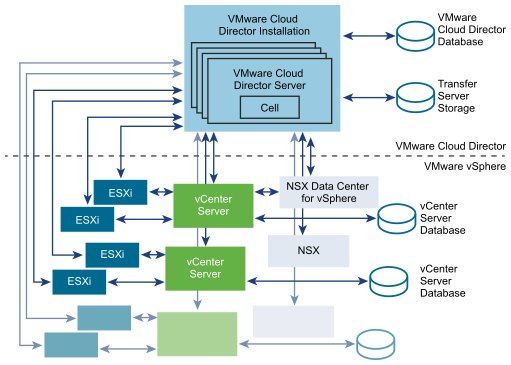
\includegraphics[scale=0.7]{figures/vcloud_components.png}
	\caption{اجزای تشکیل دهنده \lr{vCloud}\cite{mstoimenova}}
	\label{fig:vcloud_components}
\end{figure}

مهم‌ترین مولفه‌ی تشکیل‌دهنده، خدمت‌گزار \lr{vCenter} است که وظیفه‌ی مدیریت منابع مجازی در مرکزداده را بر عهده دارد. خدمت‌گزار \lr{vCenter} با فراناظر\LTRfootnote{Hypervisor} \lr{vSphere} ارتباط برقرار می‌کند تا عملیات‌های کلیدی مانند ایجاد، استقرار و مدیریت ماشین‌ها و منابع مجازی را انجام دهد.

مولفه دیگر که برای مجازی‌سازی خدمات شبکه طراحی شده‌است، سکوی \lr{NSX} است که وظیفه‌ی ارائه‌ی قابلیت‌های مجازی‌سازی شبکه به مرکزداده را بر عهده دارد. \lr{NSX} مجازی‌سازی شبکه را با ایجاد شبکه‌های ایزوله از یکدیگر فراهم می‌کند و به چندین مستأجر\LTRfootnote{Tenant} اجازه می‌دهد تا زیرساخت فیزیکی مشابهی را بدون تداخل با یک‌دیگر به اشتراک بگذارند.

مولفه‌ی مجازی‌سازی‌ خدمات ذخیره‌سازی دائم، توسط \lr{vSAN} ارائه شده‌است که یک سکو‌ی  ذخیره‌سازی نرم‌افزاری است که مشتریان را قادر می‌سازد منابع ذخیره‌سازی را در یک محیط مجازی مدیریت کنند. \lr{vSAN} به مشتریان امکان ایجاد حجم\LTRfootnote{Volume}‌های ذخیره‌سازی مجازی را می‌دهد که می‌تواند برای ذخیره‌ی فایل‌های ماشین مجازی و همچنین فضای ذخیره‌ی اشیا\LTRfootnote{Object Storage} استفاده شود.

در نهایت، سکو‌ی \lr{VMWare Cloud Director} یک رابط برنامه‌نویسی ارائه می‌کند که به مشتریان اجازه می‌دهد زیرساخت ابری خود را مدیریت کنند. این رابط برنامه‌نویسی بر پایه‌ی استاندارد \lr{REST} تعریف شده که می‌تواند برای عملیات‌های مختلف مانند ایجاد و مدیریت ماشین‌های مجازی، شبکه‌ها و حجم‌های ذخیره‌سازی استفاده شود.

\section{زبان برنامه‌نویسی}
برای پیاده‌سازی سامانه‌ی مورد نظر باید از یک زبان برنامه‌نویسی وب استفاده کنیم. با توجه به حجم بالای درخواست‌ها و فشار بر روی خدمت‌گزار، سرعت زیاد و حجم و پیچیدگی کم در منطق سامانه، از معیار‌های کلیدی انتخاب زبان برنامه‌نویسی است. یکی دیگر از این معیارها، محبوبیت و توسعه‌پذیری زبان برنامه‌نویسی در آینده برای نیازمندی‌های احتمالی و پیش‌بینی نشده است. با توجه به این معیارها، انتخاب ما برای توسعه‌ی این پروژه، زبان برنامه‌نویسی \lr{Go}\LTRfootnote{https://go.dev} است.

\subsection{زبان برنامه‌نویسی \lr{Go}}
زبان \lr{Go} یک زبان برنامه‌نویسی تابعی\LTRfootnote{Functional} است که با گذر زمان محبوبیت زیادی کسب کرده و توسط بسیاری از شرکت‌ها و توسعه‌دهندگان برای ساخت برنامه‌های کاربردی مقیاس‌پذیر\LTRfootnote{Scalable} استفاده می‌شود. این زبان برای توسعه‌ی ‌یک سرویس جامع ارائه‌ی خدمات \lr{IaaS}، مزیت‌های قابل توجه و همچنین معایبی دارد که در ادامه به شرح دقیق‌تر آن‌ها می‌پردازیم.

\clearpage

مزایای استفاده از \lr{Go} برای پیاده‌سازی یک رابط برنامه‌نویسی مقیاس‌پذیر شامل این موارد اس\cite{Lockard2019}:
\begin{enumerate}

\item  \textbf{هم‌زمانی\LTRfootnote{Concurrency} به صورت ذاتی}: یکی از برجسته‌ترین مزایای \lr{Go}، پشتیبانی قوی آن در مدیریت همزمانی است که آن را برای ساختن سیستم‌های بزرگ‌مقیاس که نیاز به استفاده‌ی کارآمد از منابع دارند، مناسب می‌کند. در یک محیط ابری که تقاضا برای منابع می‌تواند به سرعت تغییر کند، مدل پیاده‌سازی هم‌زمانی در \lr{Go}، به‌کارگیری منابع را در حالتی ایده‌آل حفظ می‌کند.


\item  \textbf{مدیریت حافظه}: \lr{Go} دارای یک جمع‌کننده زباله\LTRfootnote{Garbage Collector} داخلی است که مدیریت حافظه را آسان‌تر می‌کند و بر خلاف زبان‌های سطح پایین مانند \lr{C} و \lr{C++} این فرصت را به توسعه‌دهندگان می‌دهد تا روی عملکرد برنامه‌شان تمرکز کنند. این مورد همچنین به کاهش خطر نشت حافظه\LTRfootnote{Memory Leak} کمک می‌کند، که می‌تواند باعث ایجاد مشکلات پایداری و امنیتی شود.

\item \textbf{سادگی}: \lr{Go} دارای یک نحو\LTRfootnote{Syntax} ساده و شبیه به زبان‌های بسیار معروف \lr{C}و پایتون است که یادگیری و استفاده از آن را نسبت به زبان‌های دیگر برنامه‌نویسی آسان‌تر می‌کند.

\item \textbf{کارایی\LTRfootnote{Performance}}: \lr{Go} برای کارایی بهینه طراحی شده‌است. برای سامانه‌ها و برنامه‌هایی که باید بار پویا و در مقیاس بالا را مدیریت کنند، یک گزینه مناسب محسوب می‌شود. کامپایل شدن برنامه‌ها و اجرای مستقیم بر روی سیستم عامل در کنار  محیط اجرای بهینه، این زبان برنامه‌نویسی را از نظر زمان اجرا در کنار زبان‌های سطح پایینی همچون \lr{C++} قرار می‌دهد.\cite{Donovan2015}
\end{enumerate}

با وجود این مزیت‌ها، چالش‌هایی نیز برای استفاده از این زبان برنامه‌نویسی مطرح اس\cite{Lockard2019}. از جمله:
\begin{enumerate}
\item \textbf{محدود بودن جامعه}: باوجود محبوبیت رو به رشد این زبان برنامه‌نویسی، به دلیل سن کم‌تر نسبت به زبان‌های دیگر مانند \lr{JavaScript}، \lr{Java} و یا \lr{Python}، این زبان برنامه‌نویسی از جامعه‌ی متن‌باز کوچک‌تری برخوردار است که به سبب آن محدودیت‌هایی برای کتاب‌خانه‌ها و قطعه کد‌های خاص‌منظوره پدیدار شده است.

\item \textbf{شیب یادگیری تند}: با وجود نحو آشنا و نزدیک \lr{Go}، این زبان از اصول و ضرب‌المثل\LTRfootnote{Idiom}‌های خاصی پیروی می‌کند که ممکن است در چهارچوب‌ها و الگوهای زبان‌های دیگر حضور نداشته باشند. توسعه‌ی برنامه‌های شاخص و الگو، نیازمند رعایت این اصول است که این امر، اثرگذاری افراد با تجربه‌ی کم در توسعه‌ی برنامه‌های این زبان را کاهش می‌دهد.
\end{enumerate}

با وجود این مسائل از بین گزینه‌های موجود، انتخاب نهایی ما زبان برنامه‌نویسی \lr{Go} است.

\section{استاندارد \lr{REST}}
در تمام برنامه‌های تحت وب، یکی از کلیدی‌ترین تصمیمات در طراحی، انتخاب پروتکل و استاندارد‌های مربوط به انتقال داده و اتصال برنامه‌ به کاربر است. یکی از پرکاربردترین استانداردهای مورد استفاده در برنامه‌های تحت وب، استاندارد \lr{REST}\LTRfootnote{Representational State Transfer} است.

عملیات‌های محدود و وجود قوانین جامع، باعث سادگی تعریف و توسعه‌ی نقطه‌های دسترسی به منابع با این استاندارد شده. همچنین عدم نگهداری وضعیت بین درخواست‌ها باعث می‌شود که به سادگی بتوان برنامه‌ها را به صورت افقی نسبت به بار مقیاس کرد. با توجه به اینکه قوانین در این استاندارد کاملا مستقل از زیرساخت و سکوی توسعه و اجرا است، استفاده از این استاندارد، امکان استفاده‌ی گستره‌ی بسیار وسیعی از کاربران از خدمات را فراهم می‌آورد.\cite{Fielding:2000}

همچنین زبان \lr{Go} به صورت طبیعی از این استانداردها پیروی می‌کند و کتاب‌خانه و چهارچوب‌های متعددی از جمله چهارچوب \lr{Echo}\LTRfootnote{https://echo.labstack.com/} برای این منظور در جامعه‌ی متن‌باز این زبان، یافت می‌شود.

\section{پایگاه ذخیره داده}
برنامه‌ی ما نیازمند ذخیره‌سازی طیف گسترده‌ای از اطلاعات است. این اطلاعات شامل تنظیمات و اطلاعات مورد نیاز هر بخش از سامانه، رخداد‌ها و وقایع رخ داده در سامانه و منابع و مدل‌های مورد استفاده‌ی کاربران می‌شود. برای ذخیره‌سازی این اطلاعات، انتخاب‌های متعددی برای پایگاه داده داریم که در این پروژه بسته به ماهیت داده و نوع وابستگی برنامه به آن، از دو دسته‌ی کلی پایگاه‌های داده رابطه‌ای و غیر رابطه‌ای استفاده می‌کنیم.

\subsection{پایگاه داده رابطه‌ای}
پایگاه داده‌های رابطه‌ای، به دسته‌ای از پایگاه‌های داده گفته می‌شود که بر مبنای زبان پرسمان ساختاریافته (\lr{SQL}\LTRfootnote{Structured Query Language}) تعریف شده‌اند. در این پایگاه‌های داده، اطلاعات در جداولی با روابط تعریف‌شده، سازماندهی می‌شوند و پرسمان‌ها را می‌توان با استفاده از \lr{SQL} برای بازیابی داده‌های خاص ایجاد کرد. نمونه‌هایی از پایگاه داده‌های \lr{SQL} عبارتند از \lr{MySQL}، \lr{Oracle} و \lr{Microsoft SQL Server}. پایگاه‌های داده \lr{SQL} برای برنامه‌هایی که نیاز به تراکنش‌های پیچیده دارند و شامل مقادیر زیادی از \textbf{داده‌های ساختاریافته} هستند؛ مانند سیستم‌های مالی، سامانه‌های مدیریت کاربران و تعریف منابع با قابلبیت تغییر مکرر مناسب هستند.

بیلکمنتایسبلمنتایسمبناتیسمبناتبیسمناتیبمنبتاسیبیس (جمله بالا رو درست کن)


به طور کلی، اطلاعات ساختاریافته‌ای را که می‌‌توان در جداول با ستون‌های ثابت تعریف کرد، در این پایگاه داده ذخیره می‌کنیم. در این پروژه، ما از پایگاه داده ‌ی\lr{\textbf{PostgreSQL}}\LTRfootnote{https://www.postgresql.org/} که یکی از معروف‌ترین پایگاه داده‌های رابطه‌ای متن‌باز است استفاده می‌کنیم. 
\subsection{پایگاه داده غیر‌ رابطه‌ای}
در مقابل پایگاه‌ داده‌های رابطه‌ای، پایگاه داده‌های غیر رابطه‌ای (\lr{NoSQL}\LTRfootnote{Not Only SQL}) تعریف می‌شوند. این دسته از پایگاه‌های داده به گونه‌ای طراحی شده ‌اند که بتوانند حجم بسیار زیادی از اطلاعات نیمه ساختار یافته\LTRfootnote{Semi Structured Data} را پردازش کنند. این اطلاعات همانگونه که از مفهومش برداشت می‌شود ساختار ثابت و جدول مانند ندارد، بلکه حالت‌های متنوعی از جمله کلید-مقدار، سند پایه، گراف پایه و ستون پایه را شامل می‌شود\cite{Stonebraker2010}.

در این پروژه ما رخدادهای سامانه که ساختار یکتایی ندارند و همچنین از حجم بسیار بالایی برخوردار هستند را در پایگاه داده غیر رابطه ای ذخیره می‌کنیم. ابزاری که برای این منظور استفاده می‌کنیم پایگاه داده \lr{\textbf{MongoDB}}\LTRfootnote{https://www.mongodb.com} است که یک پایگاه داده متن‌باز است.

\section{معماری میکروسرویس}
معماری میکروسرویس\LTRfootnote{Microservice} یک الگوی طراحی\LTRfootnote{Design Pattern} محبوب است که در توسعه‌ی نرم‌افزار‌های مدرن برای ایجاد برنامه‌های کاربردی مقیاس‌پذیر، قابل نگهداری و انعطاف‌پذیر استفاده می‌شود. این معماری بر اساس ایده‌ی تجزیه‌ی یک سیستم نرم‌افزاری پیچیده به سرویس‌های کوچکتر و مستقل است که می‌توانند به طور مستقل، توسعه یافته، استقرار یابند و مدیریت شوند. این رویکرد چندین مزیت از جمله بهبود مقیاس‌پذیری، افزایش تحمل خطا و سرعت توسعه را ارائه می‌دهد.

میکروسرویس مبتنی بر مفهوم معماری سرویس‌گرا (\lr{SOA}\LTRfootnote{Service-Oriented Architecture}) است که شامل تجزیه‌ی یک سیستم نرم‌افزاری پیچیده به اجزای کوچکتر و مستقل است. با این حال، معماری میکروسرویس، این مفهوم را با تعریف هر مؤلفه به عنوان یک سرویس جداگانه که برای انجام یک عملکرد واحد طراحی شده است، یک قدم جلوتر می‌برد. این رویکرد به درجه بسیار بالاتری از انعطاف‌پذیری منجر می‌شود، زیرا هر سرویس می‌تواند مستقل از سایر سرویس‌ها مدیریت و دچار دخل و تصرف شود.

بخشی از مزایای این معماری در برنامه‌های داده‌محور\LTRfootnote{Data Driven} و رخداد‌محور \LTRfootnote{Event Driven} در زیر توضیح داده شده\cite{Hightower2017}\cite{Fowler2014}:
\begin{itemize}
\item \textbf{سرعت توسعه نرم‌افزار}: با توجه به مستقل بودن واحد‌های تعریف‌شده‌ی برنامه در این معماری، تیم‌ها و افراد مختلف می‌توانند مستقل و موازی بر توسعه سامانه کار کنند. این امر باعث افزایش قابل توجه سرعت و چابکی توسعه برنامه‌ها می‌شود. همچنین با توجه به تعریف روابط میان سرویس‌ها از قبل، اعمال و اجرای تغییرات درونی برنامه‌ها بسیار راحت‌تر و سریع‌تر انجام می‌شود.

\item \textbf{مقیاس پذیری}: به دلیل جدا و منزوی بودن سرویس‌ها در این معماری، مقیاس هر سرویس را می‌توان متناسب با بار سامانه تنظیم کرد. این مورد به این معنی است که می‌توان قسمت‌های مختلف سامانه را در هر زمان کم و زیاد یا بزرگ و کوچک کرد.

\item \textbf{تحمل خطا}: هرگونه خطا و اخلال در یک سرویس در معماری میکروسرویس، از قبل پیش‌بینی شده است و همواره می‌توان تمهیدات لازم جهت تحمل خطا را در سرویس‌های دیگر از پیش آماده کرد. همچنین اخلال در یک سرویس، فقط در همان سرویس اثرگذار است و عملکرد سایر سرویس‌های مستقل دچار اختلال نمی‌شود.

\end{itemize}

با وجود این مزایا، این معماری چالش‌ها و معایبی را نیز به دنبال دارد\cite{Hightower2017}\cite{Fowler2014} که در ادامه به بررسی آنها می‌پردازیم.

\begin{itemize}
	 \item \textbf{پیچیدگی طراحی}: هنگام طراحی میکروسرویس‌های موجود در یک سامانه، باید تمامی روابط و هماهنگی‌های میان‌سرویسی را از قبل تعریف کرد. هرگونه خطا و کاستی در این مرحله، منجر به چالش‌های اساسی در مرحله اجرا و توسعه می‌شود که برطرف کردن آنها نیازمند هزینه‌ی بیشتری است. پس باید نهایت دقت را در مرحله طراحی میکروسرویس‌ها به خرج داد.
	
	 \item \textbf{زیرساخت}: اجرا و پیاده‌سازی میکروسرویس‌ها نیازمند پیش‌نیاز‌ها و زیرساخت‌های خاص و ابزار‌های متعدد است که هزینه استفاده از این معماری را برای برنامه‌هایی با مقیاس کم و دامنه امکانات محدود، زیاد می‌کند. نیاز این معماری به تضمین زیرساخت اجرایی و شبکه‌ای از جمله‌ی این پیش‌نیازها است.
	
	 \item \textbf{حفظ سازگاری داده}\LTRfootnote{Data Consistency}: با گسترده شدن داده‌ها میان سرویس‌های مختلف و احتمال وجود خطا در هر قسم\LTRfootnote{Partition} از سامانه، تضمین سازگاری داده بدون ضمانت سلامت زیرساخت امری بسیار دشوار است.
	
	 \item \textbf{سربارهای اضافی}: استفاده از سرویس‌های متعدد برای سامانه‌ها با دامنه فعالیت‌های محدود، باعث به‌وجود آمدن سربار‌های کد، شبکه و محاسبات می‌شود.
\end{itemize}

در نهایت، براساس موارد مطرح شده، برای تصمیم‌گیری در مورد استفاده از معماری میکروسرویس، باید دامنه‌ی فعالیت‌ها، فشار ناشی از بار در قسمت‌های مختلف، محدودیت‌های تیم توسعه و محدودیت‌های زیرساخت سامانه را در نظر گرفت. با در نظر گرفتن این موارد، در این پروژه معماری مورد استفاده‌ی ما، معماری میکروسرویس است.

\section{‌دروازه‌ی ورود رابط}
الگوی طراحی ‌دروازه‌ی ورود رابط\LTRfootnote{API Gateway}، یکی از الگوهای رایجی است که در کنار میکروسرویس‌ها استفاده می‌شود. در این الگو، برنامه‌ای به عنوان یک پیش‌کار\LTRfootnote{Proxy} که وظیفه‌ی مسیریابی درخواست‌های ورودی را بر عهده دارد، قرار داده می‌شود. مدیریت بخش بزرگی از موارد امنیتی، نظارتی و سلامتی میکروسرویس‌ها بر عهده این لایه قرار می‌گیرد.

در حالت پیش‌فرض شکل\ref{fig:no-api-gateway}، کاربران سامانه مستقیما با میکروسرویس‌ها در ارتباط هستند که این امر ملاحظات جدی امنیتی و کارایی به دنبال دارد. در این حالت، تمامی میکروسرویس‌ها باید عملیات‌های مشترکی همچون احراز هویت، واقعه‌نگاری ونظارت را پیاده‌سازی کنند.


\begin{figure}[h]
	\vspace{1cm}
	\centering
	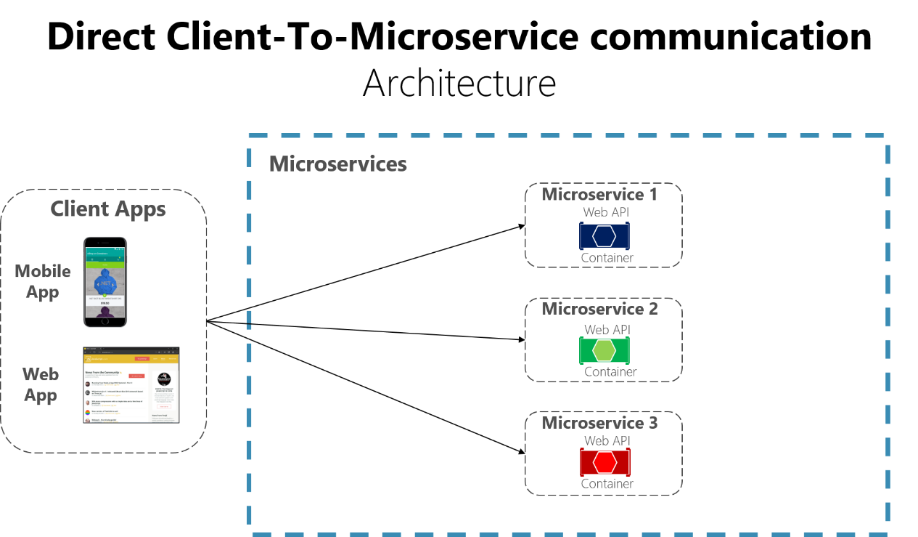
\includegraphics[scale=1]{figures/direct-client-to-microservice-communication.png}
	\caption{معماری یک سامانه میکروسرویس بدون ‌دروازه‌ی ورود رابط\cite{Microsoft_API_Gateway_2023}}
	\label{fig:no-api-gateway}
\end{figure}

در مقابل معماری شکل\ref{fig:no-api-gateway}، معماری سامانه در صورت استفاده از یک دروازه‌ی ورود رابط، مانند شکل\ref{fig:api-gateway} می‌شود. در این معماری، تعداد قابل توجهی از عملیات‌های مشترک را می‌توان در لایه ‌دروازه‌ی ورود انجام داد. به طور کلی، مزیت‌های استفاده از ‌دروازه‌ی ورود رابط را می‌توان به شکل زیر بیان کرد\cite{Microsoft_API_Gateway_2023}:

\begin{itemize}
	\item \textbf{مدیریت متمرکز}: هنگامی که دروازه‌ی مکاتبه و تعامل با تمامی کاربران سامانه ثابت و مشخص باشد، مدیریت نحوه‌ی این ارتباط کاملا مستقل از عملکرد درونی سامانه می‌شود و می‌توان نظارت و مدیریت کامل‌تری بر روی درخواست‌های کاربران و پاسخگویی به آن‌ها داشت.
	
	\item \textbf{امنیت}: با وجود یک لایه‌ی کاملا مستقل در پیش‌روی کاربر، می‌توان مکانیزم‌های امنیتی نظیر احراز هویت و مجوزها را در کنار موارد امنیت شبکه یکجا مدیریت کرد. این گونه میکروسرویس‌ها، کاملا درون یک شبکه منزوی و غیر قابل دسترس از بیرون تجمیع می‌شوند که خطر ریسک‌های امنیتی را به شکل قابل توجهی کاهش می‌دهد.
	
	\item \textbf{تقسیم بار}: لایه ‌دروازه‌ی ورود می‌تواند بار ورودی را بین نسخه‌های متعدد میکروسرویس‌ها تقسیم کند و در صورت نیاز اتصال به بخش‌های خاصی از سامانه را کمتر یا زیادتر کند.
	
\item \textbf{نظارت}: با پیاده‌سازی واحدهای نظارتی در ‌دروازه‌ی ورود، تمامی رفتار کاربران و نحوه برخورد‌ سامانه با آن‌ها را یکجا و به ‌طور متمرکز در اختیار خواهیم داشت که برای مقاصد ایرادیابی و تحلیلی فواید زیادی دارد.
\end{itemize}

\begin{figure}[h]
	\vspace{1cm}
	\centering
	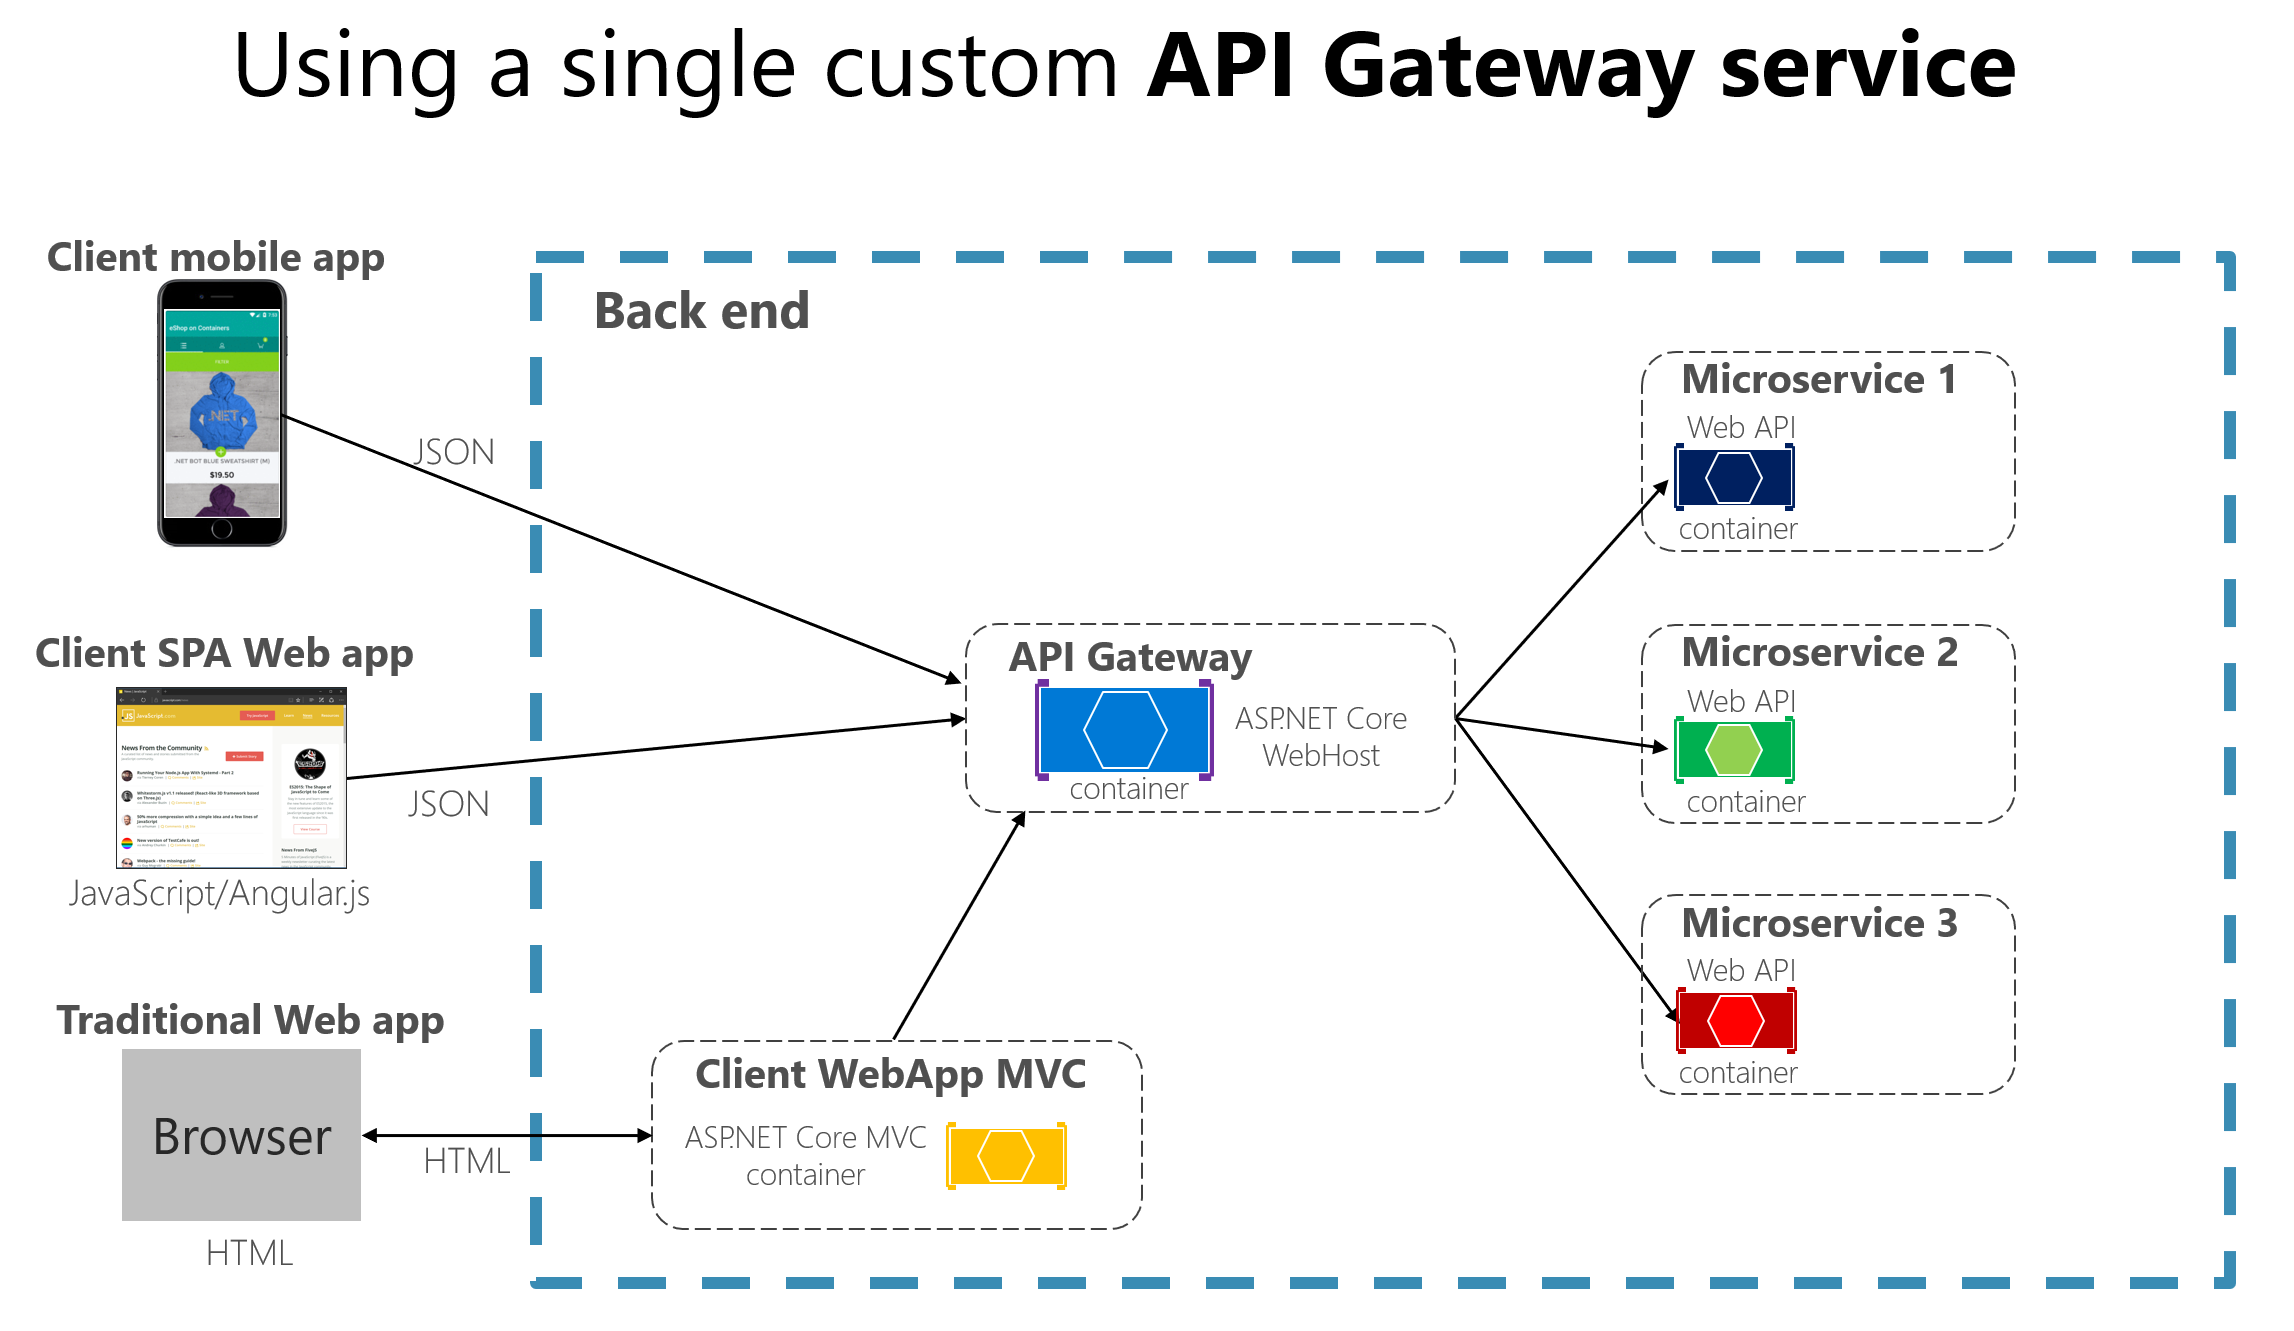
\includegraphics[scale=0.4]{figures/custom-service-api-gateway.png}
	\caption{معماری یک سامانه میکروسرویس با وجود یک ‌دروازه‌ی ورود رابط\cite{Microsoft_API_Gateway_2023}}
	\label{fig:api-gateway}
\end{figure}

\section{داکر}
داکر\LTRfootnote{Docker} یکی از کاربردی‌ترین ابزار‌ها برای پیاده‌سازی معماری میکروسرویس است. این ابزار که خود از چندین بخش تشکیل شده، امکان بسته‌بندی برنامه‌ها در واحد کانتینر\LTRfootnote{Container} را فراهم می‌کند و کاربران می‌توانند این کانتینر‌ها را در یک موتور کانتینر\LTRfootnote{Container Engine} مثل موتور داکر\LTRfootnote{Docker Engine} اجرا کنند. با انجام این کار، کانتینرها به صورت مستقل از یکدیگر در یک محیط منزوی اجرا می‌شوند. فواید این مدل اجرا، شامل مقیاس پذیری راحت، قابل حمل بودن واحد‌های اجرایی برنامه، سازگاری و انعطاف پذیری نسبت به محیط اجرا و ابزار‌ها است. معماری کلی داکر و فرایند عملکرد این ابزار در شکل\ref{fig:docker-arch} مشخص شده است. کاربران با استفاده از برنامه \lr{docker} 
با سرویس \lr{docker daemon} که همواره در پس‌زمینه در‌حال اجرا است، در تعامل‌ خواهند بود. این برنامه سپس تصاویر\LTRfootnote{Images} را از مخزن محلی و یا مرکزی دریافت کرده و در قالب کانتینرهای موتور داکر اجرا‌ می‌کند.
\begin{figure}[h]
	\vspace{1cm}
	\centering
	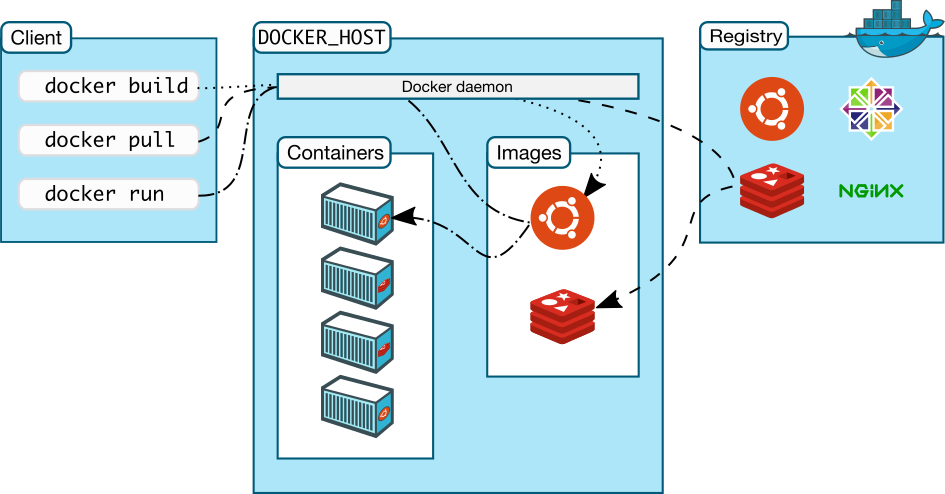
\includegraphics[scale=0.4]{figures/docker-architecture.png}
	\caption{معماری داکر}
	\label{fig:docker-arch}
\end{figure}

تفاوت کانتینرهای داکر با ماشین‌های مجازی که در گذشته به همین منظور استفاده می‌شدند در شکل\ref{fig:docker-container-vm}‌ قرار گرفته. برخلاف ماشین مجازی، کانتینرها توسط موتور کانتینر (در این شکل موتور داکر) بر روی سیستم عامل میزبان اجرا می‌شوند. این مدل اجرا، باعث از بین  رفتن سربارهای مجازی سازی دستورات و سخت افزار می‌شود.

\begin{figure}[h]
	\vspace{1cm}
	\centering
	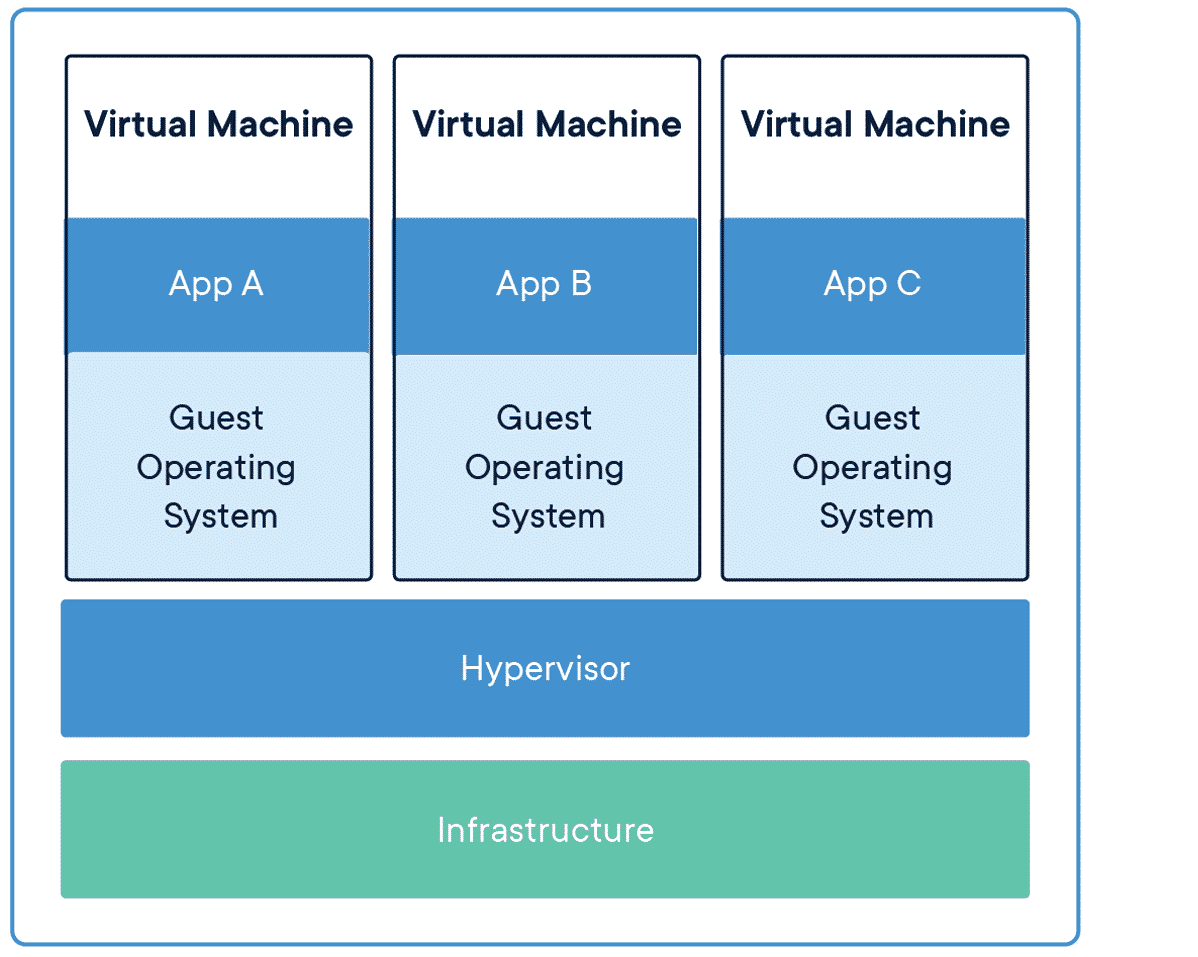
\includegraphics[scale=0.17]{figures/container-vm-whatcontainer.png}
	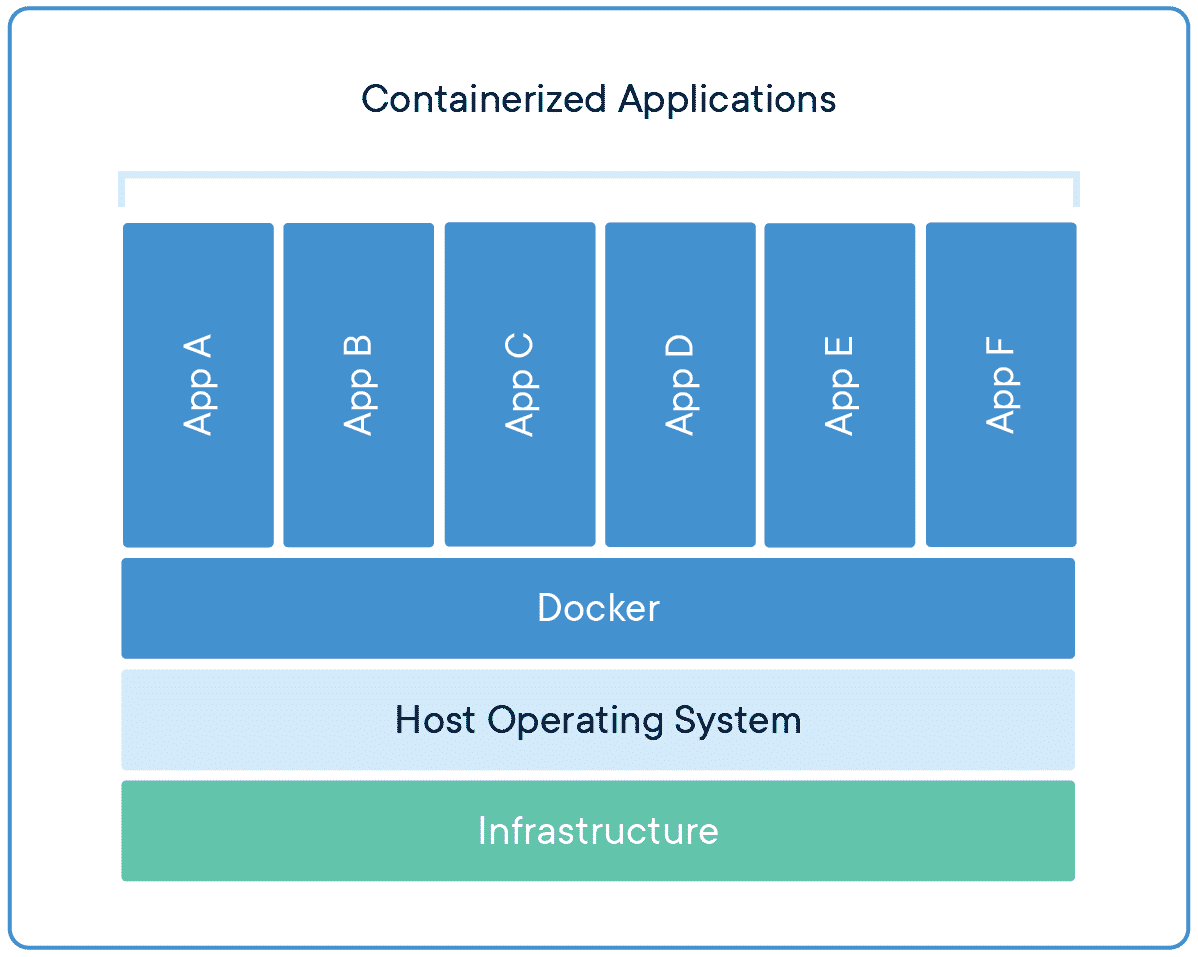
\includegraphics[scale=0.17]{figures/docker-containerized-appliction-blue-border.png}
	\caption{لایه‌های کانتینر داکر}
	\label{fig:docker-container-vm}
\end{figure}


\section{نتیجه گیری}

در این پروژه، ما به عنوان زیرساخت ارائه خدمات \lr{IaaS} از سرویس \lr{VMWare Cloud Director} بهره گرفتیم.برای سرویس‌های مورد نیاز برای توسعه خدمات، از زبان برنامه‌نویسی \lr{Go} و از چهارچوب‌ها و کتاب‌خانه‌های این زبان استفاده کردیم. رابط‌های سامانه با کاربران بیرون و تعاملات درونی سامانه از استاندارد \lr{REST} پیروی می‌کنند و کتاب‌خانه \lr{Echo} در زبان برنامه‌نویسی \lr{Go} برای پیاده‌سازی این موضوع به کار گرفته شده. برای ذخیره داده از تکنولوژی‌های پایگاه داده رابطه‌ای و غیر رابطه‌ای استفاده کردیم. راه اندازی پایگاه داده رابطه‌ای با ابزار \lr{PostgreSQL} است و برای پایگاه داده غیر رابطه‌ای از ابزار \lr{MongoDB} استفاده کرده‌ایم.

پیاده‌سازی سرویس‌ها در قالب معماری میکروسرویس شد که تمامی قسمت‌های سامانه در قالب تصاویر داکر قرار گرفتند. این سرویس‌ها داخل یک شبکه داخلی پشت یک ‌دروازه‌ی ورود رابط جای گرفتند که این ‌دروازه‌ی ورود رابط، وظیفه‌های نظارت، احراز هویت و ثبت وقایع را برعهده دارد.
\chapter{طراحی و پیاده‌سازی سیستم}
در این فصل، به مراحلی که برای پیاده‌سازی این سیستم طی شده‌است، پرداخته شده‌است.


\section{طراحی و معماری سیستم}
با توجه به نیازمندی‌های مطرح شده برای خدمات سامانه، در ابتدا باید دامنه‌ی فعالیت‌های بخش‌های مختلف سامانه را مشخص کنیم. این تصمیم گیری باید به گونه‌ای باشد که بخش‌ها، کمترین وابستگی و جفت شدگی\LTRfootnote{Coupling} را داشته باشند.

با توجه به استقلال نیازمندی‌ها و عملکرد‌های ذکر شده برای سامانه، معماری کلی این سامانه، معماری میکروسرویس است. در این پیاده‌سازی، هر نیازمندی در یک سرویس پیاده‌سازی شده است، یک سرویس جهت انجام امور احراز هویت، یک سرویس برای تعامل با کاربران و تحویل درخواست‌های آنان، یک سرویس جهت تعامل با زیرساخت ابری جهت اجرای دستورات و در نهایت یک سرویس جهت امور نظارتی و مدیریتی تعریف شده که همه این سرویس‌ها در یک شبکه‌ی خصوصی و پشت سر یک ‌دروازه‌ی ورود رابط قرار گرفته. معماری کلی سامانه در شکل\ref{fig:30bird-arch} مشخص شده است. در ادامه‌ی این فصل جزئیات هر بخش از این معماری را دقیق‌تر بررسی می‌کنیم.

\begin{figure}
	\centering
	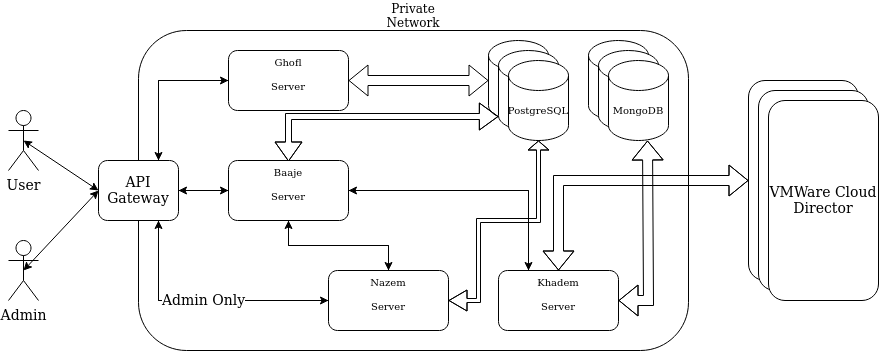
\includegraphics[scale=0.5]{figures/30bird-arch.png}
	\caption{معماری کلی سامانه}
	\label{fig:30bird-arch}
\end{figure}


\clearpage
\section{میکروسرویس‌ها}
کل سامانه از چهار میکروسرویس تشکیل شده: قفل، ناظم، خادم و باجه. هر میکروسرویس، مخصوص رسیدگی به امور بخشی از سامانه است. این میکروسرویس‌ها در قالب معماری کد تک مخزنه\LTRfootnote{Mono Repo} پیاده‌سازی شده‌اند و دارای اشتراک‌های زیادی در کد‌های پایه هستند.

\subsection{جزئیات فنی مشترک}
در این بخش قصد داریم که این موارد مشترک را مطرح کنیم و سپس به بررسی جزئیات اختصاصی هر سرویس بپردازیم.

این موارد شامل:

\begin{itemize}
	\item خدمت‌گزار وب
	\item برنامه‌ی تحت خط‌‌فرمان
	\item مدیریت تنظیمات
	\item تعامل با پایگاه داده و مدیریت مدل‌ها
	\item ساختار کد
\end{itemize}
می‌شود که در ادامه‌ی این بخش به شرح جزئیات هر‌یک می‌پردازیم.


اجرای یک خدمت‌گزار وب\LTRfootnote{Web Server} توسط چهارچوب \lr{Echo} در زبان \lr{Go} انجام می‌شود. نحوه عملکرد این چهارچوب به این شکل است که در ابتدا قوانین مربوط به مسیریاب\LTRfootnote{Router} تنظیم می‌شود، سپس برای هر مقصد\LTRfootnote{Endpoint}، یک رسیدگی کننده\LTRfootnote{Handler} تعریف می‌کنیم. به عنوان مثال برای عملیات ورود کاربر به سامانه، برای مسیر \lr{/api/login} یک رسیدگی کننده تعریف می‌کنیم که عملیات لازم جهت ورود کاربر را اجرا می‌کند. این عملیات در این مثال شامل چک کردن ورودی درخواست، اتصال به پایگاه داده، چک کردن صحت اطلاعات فرستاده شده و ارسال یک کلید ورود برای کاربر است که همگی در قالب یک تابع به عنوان رسیدگی کننده‌ی این مقصد تعریف می‌شوند. همچنین در تمامی خدمت‌گزار‌های این سامانه، کاربران بایستی هویت خود را از طریق سربرگ‌های اجباری از پیش تعیین شده مشخص کنند و یک احراز هویت با کلید ثابت انجام دهند. این امر جهت بالا بردن امنیت دوچندان سامانه تعبیه شده‌است.
در ساختار کد این پروژه، ثبت این مقصدها به همراه توابع رسیدگی کننده در بسته \lr{api/http/handler} انجام می‌شود. جهت ثبت یک بسته جدید فقط کافیست که مشخصات مقصد و تابع رسیدگی کننده در فایلی داخل این بسته نوشته شود و با تابع \lr{RegisterEndpoints} مقصد مورد نظر داخل مسیریاب \lr{Echo} ثبت شود.

معماری کلی عملکرد \lr{Echo} در شکل\ref{fig:echo-workflow} و پوشه‌بندی موارد گفته شده در شکل\ref{fig:echo-folder-router} و \ref{fig:echo-folder-handler} توضیح داده شده‌است.

\begin{figure}
	\centering
	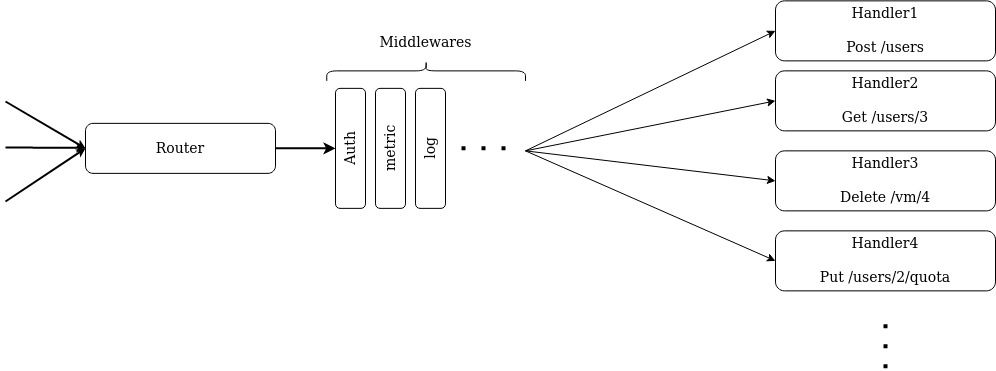
\includegraphics[scale=0.45]{figures/echo-workflow.jpeg}
	\caption{عملکرد چهارچوب \lr{Echo}}
	\label{fig:echo-workflow}
\end{figure}

\begin{figure}
	\vspace{1cm}
	\centering
	\begin{minipage}[b]{0.5\textwidth}
		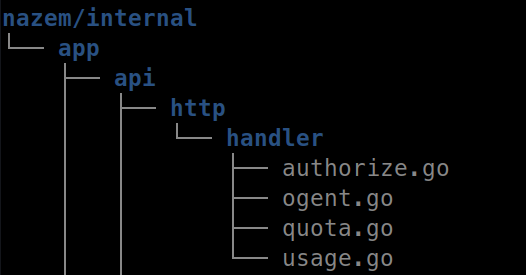
\includegraphics[width=\textwidth]{figures/echo-handler-dir.png}
		\caption{پوشه‌بندی توابع رسیدگی‌کننده \lr{Echo}}
		\label{fig:echo-folder-handler}
	\end{minipage}
	\hfill
	\begin{minipage}[b]{0.4\textwidth}
		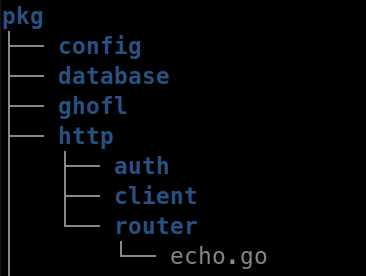
\includegraphics[width=\textwidth]{figures/echo-router-dir.png}
		\caption{پوشه‌بندی مسیریاب \lr{Echo}}
		\label{fig:echo-folder-router}
	\end{minipage}
	
\end{figure}


ایجاد برنامه‌های تحت خط‌فرمان\LTRfootnote{Command Line Application} توسط چهارچوب \lr{Cobra} پیاده‌سازی شده‌است. این چهارچوب به برنامه‌نویسان این اختیار ‌را می‌دهد که برای برنامه‌های خود یک رابط خط فرمان\LTRfootnote{Command Line Interface} ایجاد کنند. با این کار، برنامه‌نویس می‌تواند با کد‌های نوشته شده برای پروژه، چندین فرمان قابل اجرا ایجاد کند. مزیت این‌کار در سناریو‌هایی که برنامه‌ی‌ نوشته شده نیاز به اجرای چند فرمان مختلف به طور همزمان در پس‌زمینه داشته باشد مشخص می‌شود.

برنامه ‌های خط فرمان طبق پوشه‌بندی شکل\ref{fig:cobra-dir} در پروژه‌ها قرار گرفته‌اند.

\begin{figure}
	\vspace{1cm}
	\centering
	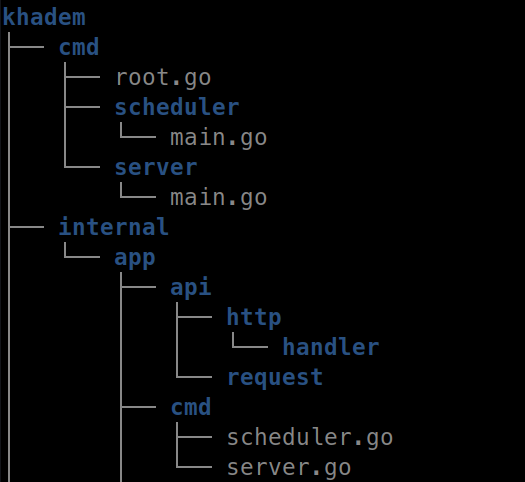
\includegraphics[scale=0.45]{figures/cobra-dir.png}
	\caption{ساختار پوشه‌بندی برنامه‌های خط فرمان در پروژه خادم}
	\label{fig:cobra-dir}
\end{figure}

مدیریت تنظیمات برنامه توسط چهارچوب \lr{Viper} انجام می‌شود. این چهارچوب، به کاربران این اجازه را می‌دهد که تنظیمات را در هر‌یک از ساختارهای معروف \lr{JSON}، \lr{YAML} و یا \lr{TOML} بنویسد و با قراردادن آن در یکی از آدرس‌های پیشفرض تنظیمات، آن‌ها را بر روی برنامه اعمال کند. ساختار انتخابی ما برای تنظیمات به صورت پیش‌فرض، ساختار \lr{YAML} است که در یک فایل هم‌اسم پروژه، در پوشه ریشه پروژه قرار گرفته.

تنظیمات برنامه می‌تواند در یکی از آدرس‌های زیر باشد.
\begin{enumerate}
	\item \lr{./<appname>.yaml}
	\item \lr{/etc/<appname>/<appname>.yaml}
	\item \lr{~/.config/<appname>.yaml}
\end{enumerate}


تعامل و ارتباطات با پایگاه داده در اپلیکیشن‌ها با دو چهارچوب \lr{gorm} و \lr{ent} انجام می‌شود. مزیت چهارچوب \lr{gorm}، سادگی عملکرد و گستردگی پشتیبانی و جامعه متن‌باز آن است. هر دو چهارچوب به عنوان یک \lr{ORM}\LTRfootnote{Object-Relation Mapping} تعامل با پایگاه داده را بسیار ساده‌تر می‌کنند. به گونه‌ای که برای ارتباط با پایگاه‌داده به هیچ‌عنوان دغدغه‌ی نحوه تعریف روابط و ذخیره‌سازی اطلاعات را نداریم و فقط با مدل‌های تعریف شده‌ی داخل برنامه تعامل برقرار می‌کنیم. در کد این پروژه، ارتباطات با پایگاه داده جهت دریافت و ثبت اطلاعات در یک لایه‌ی کاملا مجزا با استفاده از الگوی شیئ دسترسی داده\LTRfootnote{Data Access Object} پیاده‌سازی شده است. این الگوی طراحی به نویسندگان کد این امکان را می‌‌دهد، که توابع و نیازمندی‌های دسترسی به داده ذخیره‌شده را در یک لایه‌ی کاملا جداگانه تعریف کنند و لایه‌های دخل و تصرف داده را در کنار این لایه توسعه دهند\cite{oracle_dao}.

با توجه به این‌که چهارچوب \lr{ent} توسط تولید کد رابط‌های مورد نیاز جهت تعامل با پایگاه داده را فراهم می‌کند، تمامی ریسک‌ها و خطر‌های امنیتی مربوط به پایگاه داده به علت \lr{Type Safe} بودن این رابط قابل کنترل می‌شود. این مورد یکی از مزیت‌های بسیار بزرگ استفاده از این چهارچوب است.

تمامی کد‌های مربوط به تعامل با پایگاه داده مطابق شکل\ref{fig:ent}، در پوشه \lr{ent} قرار گرفته‌است. جزئیات مهم این پوشه‌بندی به شرح زیر می‌باشد.

\begin{itemize}
	\item \lr{\textbf{schema}}: این پوشه شامل تعاریف ساختار مدل‌ها در پایگاه داده است.
	\item \lr{\textbf{entc.go}}: در این فایل، قوانین تولید و تفسیر \lr{API} تعامل با پایگاه داده قرار داده شده است.
	\item \lr{\textbf{generate.go}}: این فایل، نحوه تولید فایل‌های خودکار تولید‌شده را مشخص می‌کند.
	\item \lr{\textbf{openapi.json}}: این فایل، ساختار و مشخصات \lr{API} تولید‌شده را بر اساس استاندارد \lr{OpenAPI} مشخص می‌کند.
\end{itemize}

\begin{figure}
	\vspace{1cm}
	\centering
	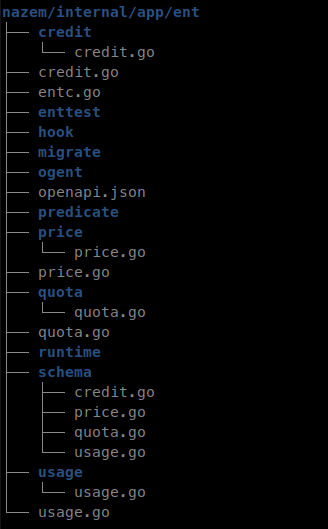
\includegraphics[scale=0.45]{figures/ent.png}
	\caption{ساختار پوشه‌بندی چهارچوب \lr{ent}}
	\label{fig:ent}
\end{figure}

با توجه به استفاده از الگوی تک‌مخزنه در نگهداری کد‌های پروژه، تا حد ممکن کد‌ها و منابع مشترک پروژه در پوشه \lr{pkg} نگهداری می‌شود. 

ساختار این پوشه در شکل\ref{fig:pkg-dir} مشخص شده، توضیحات پوشه‌های موجود در این ساختار به شرح زیر می‌باشد.
\begin{itemize}
	\item \lr{\textbf{config}}: نحوه خوانده شدن تنظیمات و قوانین مربوط به پردازش تنظیمات که بین پروژه‌ها مشترک است در فایل‌های این پوشه نوشته شده‌است.
	\item \lr{\textbf{database}}: کد‌های مربوط به نحوه اتصال به پایگاه داده و مکانیزم‌های تلاش مجدد در فایل‌های این پوشه قرار داده شده، در صورت نیاز به پشتیبانی از پایگاه داده جدید، فقط کافیست نحوه اتصال به پایگاه داده را داخل این پوشه مشخص کنیم.
	\item \lr{\textbf{http}}: میان‌افزارهای مشترک، تنظیمات مسیریاب اولیه برنامه، به همراه فایل‌های کاربر\LTRfootnote{Client}‌های برنامه‌ها در این پوشه تعبیه شده‌است.
	\item \lr{\textbf{log}}: تنظیمات مربوط به راه‌اندازی ثبت کننده وقایع در این پوشه انجام می‌شود.
	\item \lr{\textbf{model}}: مدل‌های مشترک نظیر ماشین مجازی یا تنظیمات آن در هر یک داخل فایلی داخل این پوشه قرار داده می‌شود.
\end{itemize}

\begin{figure}
	\vspace{1cm}
	\centering
	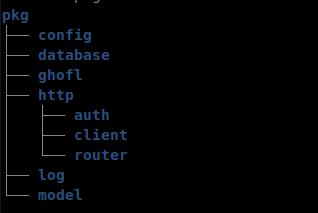
\includegraphics[scale=0.55]{figures/pkg-dir.png}
	\caption{ساختار پوشه‌بندی \lr{pkg}}
	\label{fig:pkg-dir}
\end{figure}

\subsection{قفل}
میکروسرویس مخصوص احراز‌ هویت و تعیین سطح دسترسی در این سامانه، قفل نام دارد. دلیل نام‌گذاری این میکروسرویس به این اسم، شباهت عملکرد قفل و این سامانه است که هر دو وظیفه کنترل دسترسی به منابع پشت قفل را دارند.

\begin{figure}
	\vspace{1cm}
	\centering
	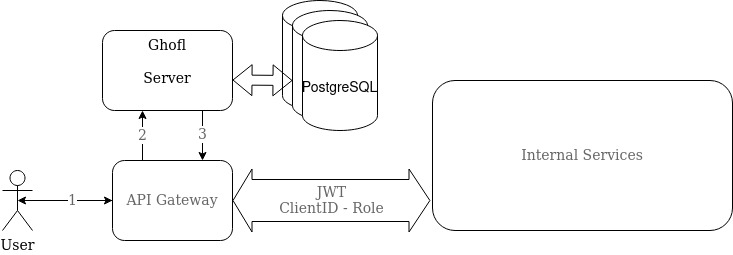
\includegraphics[scale=0.5]{figures/30bird-ghofl.jpg}
	\caption{عملکرد سرویس قفل}
	\label{fig:30bird-ghofl}
\end{figure}

در شکل\ref{fig:30bird-ghofl}، کاربرد سرویس قفل در سامانه مشخص شده‌است. \textbf{تمامی درخواست‌های ورودی} به سامانه در ابتدا به سرویس قفل فرستاده می‌شوند و احراز هویت آن‌ها انجام می‌شود. این درخواست‌ها یا مانند درخواست ورود و ثبت‌نام ماهیت احراز هویت دارند و یا سایر درخواست‌های کاربری و مدیریتی هستند. دسته اول درخواست‌ها مستقیما به قفل فرستاده می‌شوند. دسته دوم درخواست‌ها نیز هنگام رسیدن به دروازه ‌ورود، ابتدا به قفل فرستاده می‌شوند که سرایند احراز هویت \lr{JWT}\LTRfootnote{JSON Web Token} آنها ارزیابی شود. پس از این ارزیابی، در صورت موفقیت آمیز‌بودن. درخواست به سرویس‌های بالادستی فرستاده شده و درصورت ورود ناموفق کاربر با خطا مواجه خواهد شد.


پوشه بندی این پروژه در شکل\ref{fig:30bird-ghofl-dir} مشخص شده است. 
در این پوشه‌بندی، پوشه \lr{auth} مربوط به منطق‌های لازم جهت پیاده سازی احراز هویت است. 

\begin{figure}
	\vspace{1cm}
	\centering
	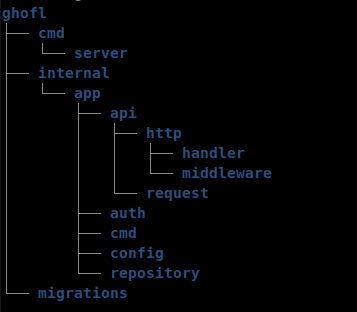
\includegraphics[scale=0.5]{figures/ghofl-dir.png}
	\caption{پوشه بندی سرویس قفل}
	\label{fig:30bird-ghofl-dir}
\end{figure}

\subsection{ناظم}
میکروسرویس ناظم وظیفه نظارت و مدیریت امور مالی و گزارشات مصرف کاربران را برعهده دارد. این میکروسرویس یکی از کلیدی‌ترین سرویس‌های سامانه است که در تعامل زیاد با پایگاه داده است. معماری کلی این سرویس در شکل\ref{fig:30bird-nazem} مشخص شده‌است.

ناظم در \textbf{تعامل با باجه} در جایگاه یک اعتبارسنج\LTRfootnote{Validator} درخواست عمل می‌کند. به این صورت که تمامی درخواست‌های مربوط به دخل و تصرف در منابع باید ابتدا از این سامانه تاییدیه بگیرند. گرفتن این تاییدیه به معنی اعتبار کافی و نبودن محدودیت بر روی کاربر برای منابع درخواستی است. هرگونه ایراد و خطا در این سرویس منجر توقف عملکرد کل سامانه است که این امر یک موضوع پیش‌بینی شده و قابل قبول است. کد‌های مربوط به این اعتبار سنجی داخل بسته \lr{validation} قرار گرفته و برای توسعه و تغییر این قوانین باید این بسته دچار تغییر شود.

در تعامل با ‌دروازه‌ی ورود، درخواست‌های مدیر سامانه جهت تغییر محدودیت‌های کاربران یا گزارش گیری از وضعیت آنان را دریافت می‌کند و پاسخ مناسب را با توجه به اطلاعات ثبت شده در پایگاه داده می‌دهد.

این سرویس برای درخواست‌های دریافتی از سرویس خادم، گزارش مصرف منابع را برای منابع دریافت می‌کند و با توجه به قوانین و قیمت گذاری‌های ثبت‌شده، اعتبار کاربر را تحت تاثیر قرار می‌دهد.

\begin{figure}
	\vspace{1cm}
	\centering
	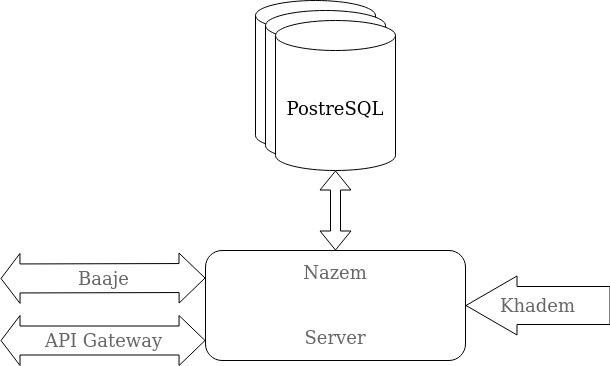
\includegraphics[scale=0.7]{figures/30bird-nazem.jpg}
	\caption{عملکرد سرویس ناظم}
	\label{fig:30bird-nazem}
\end{figure}

پوشه‌بندی بسته ها در این پروژه در شکل\ref{fig:30bird-nazem-dir} مشخص شده‌است. در این پوشه‌بندی، بسته‌ی \lr{billing} شامل منطق‌های لازم جهت صحت‌سنجی درخواست‌های تغییر منابع می‌باشد که داخل توابع رسیدگی‌کننده به همین‌نام استفاده شده

بسته‌ی مهم دیگر، بسته \lr{usage} می‌باشد که قوانین مربوط به نحوه ثبت و بروزرسانی مصرف منابع کاربر در آن تعریف و پیاده‌سازی شده‌است.

\begin{figure}
	\vspace{1cm}
	\centering
	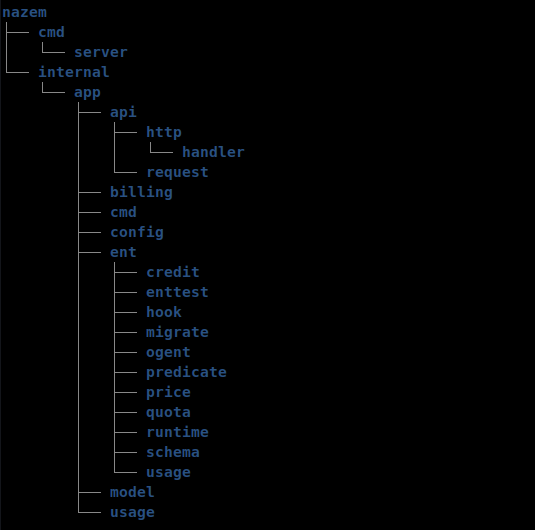
\includegraphics[scale=0.8]{figures/nazem-dir.png}
	\caption{پوشه بندی سرویس ناظم}
	\label{fig:30bird-nazem-dir}
\end{figure}


\subsection{باجه}
این سرویس دروازه ارتباطی کاربران عادی سامانه است. تمامی درخواست‌ها و عملیات ممکن برای کاربر در این برنامه قرار گرفته. معماری این برنامه در شکل\ref{fig:30bird-baaje} مشخص شده است. همانطور که در تصویر مشخص شده، این سرویس مستقیما از طریق ‌دروازه‌ی ورود با کاربران در ارتباط است و برای انجام امور مربوط به کاربران با سرویس‌های خادم و ناظم به صورت داخلی در ارتباط است.


این سرویس اطلاعات مربوط به منابع تعریف شده برای کاربر را داخل پایگاه داده ذخیره کرده و در پردازش درخواست‌ها از این اطلاعات استفاده می‌کند. منابع تعریف شده داخل پایگاه داده شده داخل پیوست این گزارش موجود است.

در مواجه با درخواست‌های مربوط به تغییر منابع مانند ساخت یا ویرایش ماشین مجازی، ابتدا اعتبارسنجی درخواست از طریق سرویس ناظم انجام می‌شود و در صورت موفقیت‌آمیز بودن این اعتبارسنجی، درخواست جهت اجرا به سرویس خادم ارسال می‌شود. پس از رسیدن جواب از سمت سرویس خادم، بسته به خروجی سرویس خادم، نتیجه درخواست کاربر داخل پایگاه داده ذخیره می‌شود.

این قابلیت‌ها توسط بسته‌بندی‌ای که در شکل\ref{fig:30bird-baaje-dir} مشخص شده پیاده‌سازی شده‌اند. اکثر کد‌های این سرویس داخل بسته \lr{handler} قرار‌دارد که با بسته‌های کاربر بقیه سرویس‌ها، با آن‌ها به تعامل می‌پردازد.
بسته دیگری که مختص این پروژه می‌باشد، بسته \lr{validate} است که یک رابط برای سرویس ناظم است، در صورت تقسیم شدن سرویس ناظم  و یا تغییر منطق صحت‌سنجی درخواست‌ها فقط باید محتوی این بسته را تغییر داد و توابع رسیدگی کننده بدون تغییر خواهندبود.
\begin{figure}
	\centering
	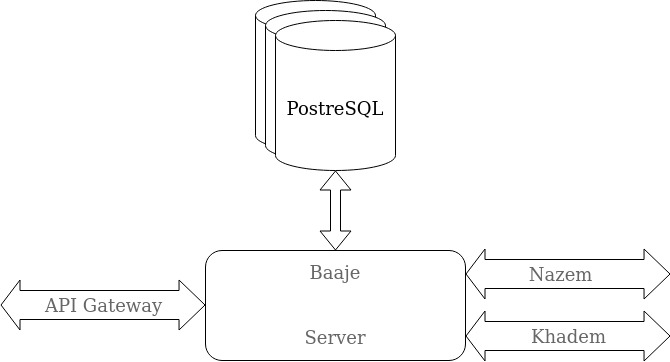
\includegraphics[scale=0.5]{figures/30bird-baaje.jpg}
	\caption{عملکرد سرویس باجه}
	\label{fig:30bird-baaje}
\end{figure}

\begin{figure}
	\vspace{1cm}
	\centering
	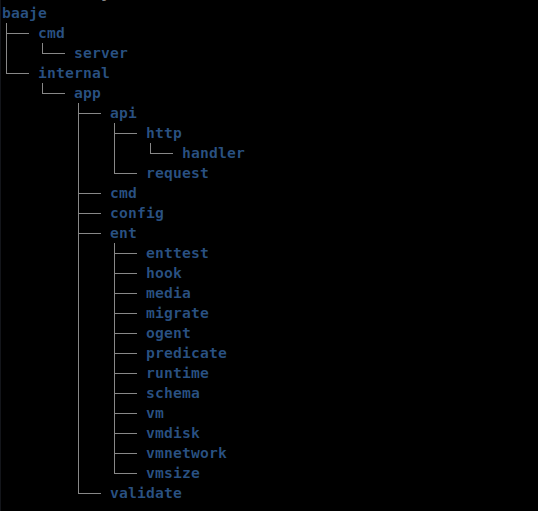
\includegraphics[scale=0.7]{figures/baaje-dir.png}
	\caption{پوشه بندی سرویس باجه}
	\label{fig:30bird-baaje-dir}
\end{figure}


\begin{figure}
	\vspace{1cm}
	\centering
	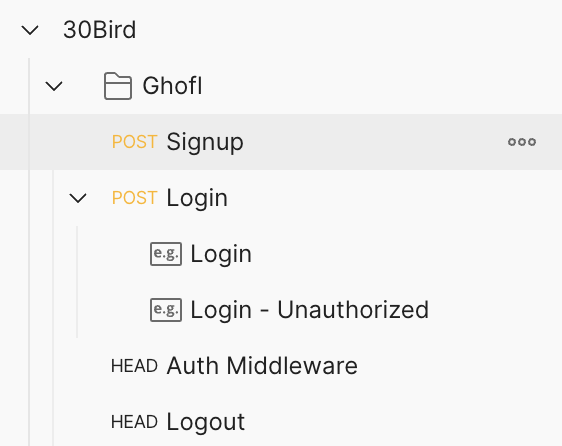
\includegraphics[scale=0.7]{figures/ghofl-api.png}
	\caption{لیست \lr{Endpoint}های سرویس قفل}
	\label{fig:ghofl-api}
\end{figure}


\begin{figure}
	\vspace{1cm}
	\centering
	\begin{minipage}[b]{0.45\textwidth}
		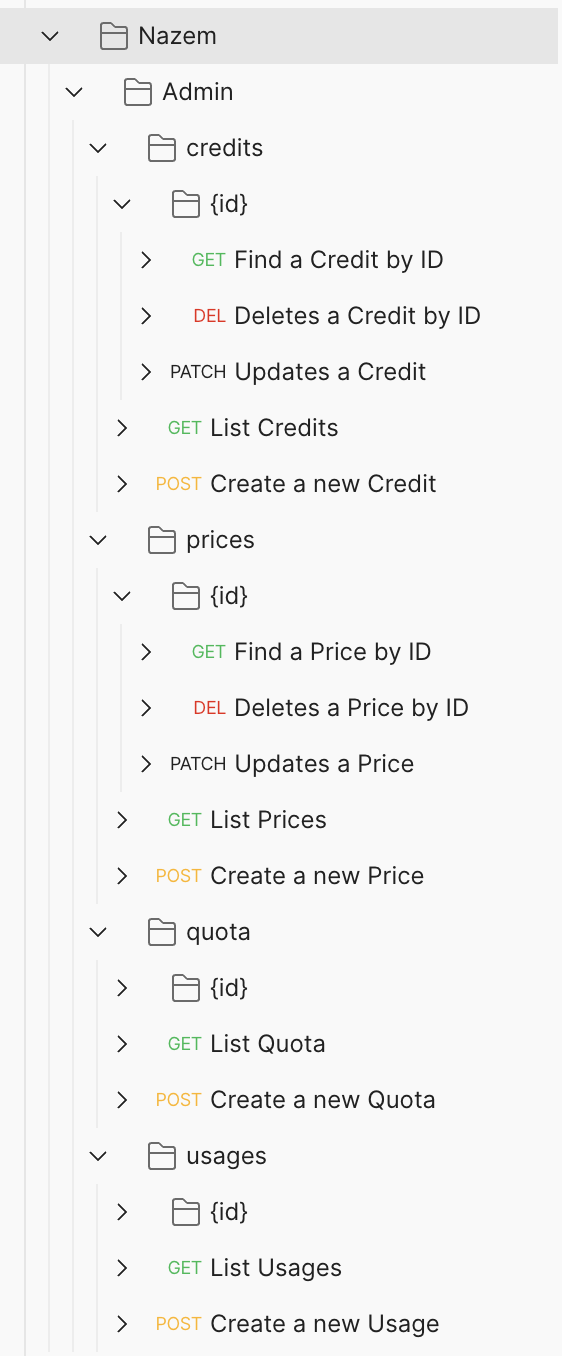
\includegraphics[width=\textwidth]{figures/nazem-api.png}
		\caption{لیست \lr{Endpoint}های سرویس ناظم}
		\label{fig:nazem-api}
	\end{minipage}
	\hfill
	\begin{minipage}[b]{0.45\textwidth}
		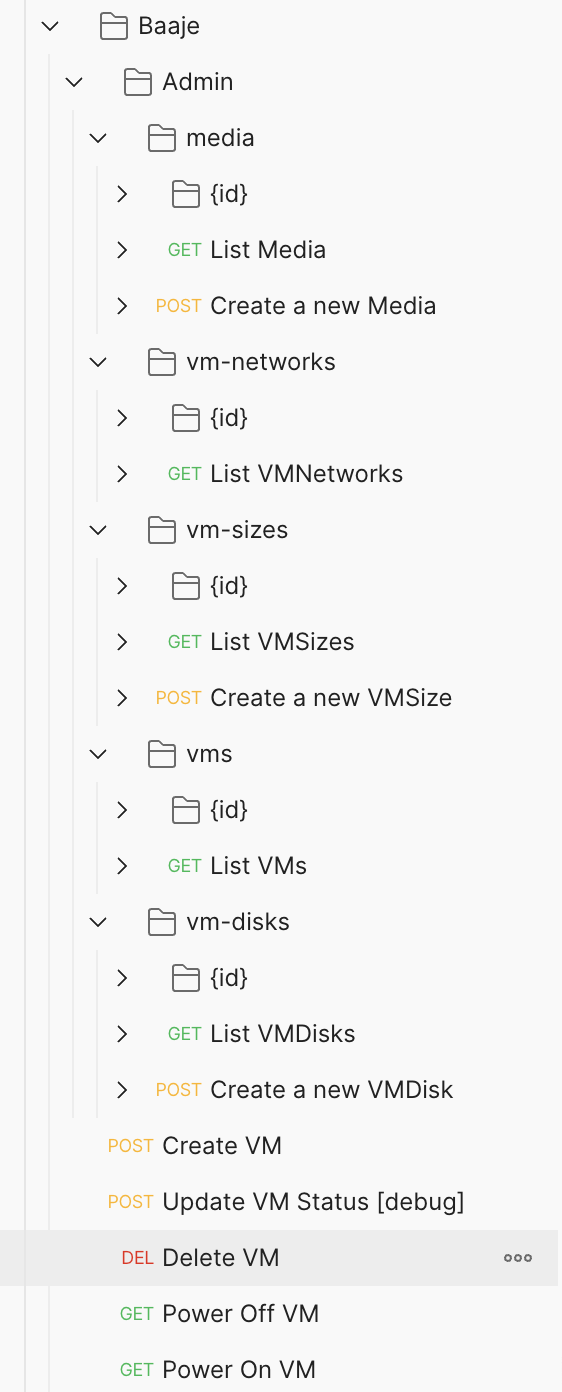
\includegraphics[width=\textwidth]{figures/baaje-api.png}
\caption{لیست \lr{Endpoint}های سرویس باجه}
\label{fig:baaje-api}
	\end{minipage}
	
\end{figure}


\clearpage
\subsection{خادم}
همانطور که قبلا گفته شد، سامانه برای ارائه خدمات \lr{IaaS} نیازمند تعامل با یک ارائه دهنده زیرساخت است. این ارائه دهنده در سامانه‌ما \lr{VMWare Cloud Director} است، میکروسرویس مسئول جهت تعامل با این برنامه خادم است. معماری خادم از دو قسمت اصلی تشکیل شده است. \textbf{خدمت‌گزار} و \textbf{زمان‌بند}\LTRfootnote{Scheduler} دو بخش تشکیل دهنده این سرویس می‌باشند که کاملا مستقل و جداگانه اجرا می‌شوند. وظیفه خدمت‌گزار دریافت دستورات از سرویس باجه و سپس تفسیر و اجرای آن‌‌ها است. معماری کلی این پروژه در شکل \ref{fig:30bird-khadem}مشخص شده است.

بسته‌بندی پروژه در شکل\ref{fig:30bird-khadem-dir} مشخص شده‌است.

\begin{figure}
	\vspace{1cm}
	\centering
	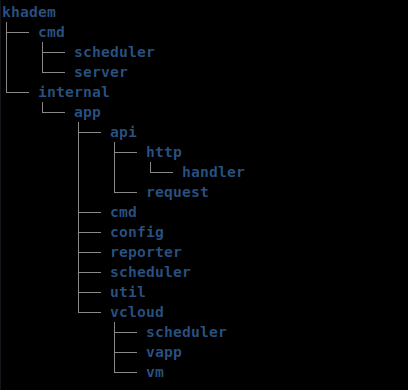
\includegraphics[scale=0.7]{figures/khadem-dir.png}
	\caption{پوشه بندی سرویس خادم}
	\label{fig:30bird-khadem-dir}
\end{figure}

پایه کد این پروژه به طور کلی در بسته \lr{vcloud} قرار داده شده‌است. این بسته شامل تمامی عملیات قابل اجرا بر روی \lr{cloud director} است. در صورت نیاز به تکمیل و یا توسعه خدمات بایستی دستورات و توابع این بسته را تغییر داد. داخل این بسته از بسته توسعه نرم‌افزار (\lr{SDK}\LTRfootnote{Software Development Kit}) رسمی \lr{VMWare Cloud Director} استفاده شده‌است. البته برای کاربرد‌های خاص و عملیات تخصصی دقیق، ممکن است که نیاز به تعامل مستقیم با \lr{API} داشته باشیم. ولی برای خدمات فعلی سامانه، تمامی امکانات مورد نیاز داخل \lr{SDK} موجود است.

منطق‌های مربوط به نظارت کننده منابع که وظیفه گزارش مصرف منابع‌ را بر عهده دارد، در بسته \lr{scheduler} قرار دارد. در این بسته یک اجراشونده کار در پس زمینه فراخوانی شده و عملیات دریافت وضعیت منابع و ارسال این اطلاعات به سرویس ناظم را انجام می‌دهد.

پوشه مهم دیگر داخل پروژه، پوشه \lr{reporter} است. این پوشه وظیفه اطلاع‌رسانی وضعیت نهایی درخواست‌های ارسال شده به خادم  به سرویس‌های بالادستی را برعهده دارد. از نمونه‌ی این اطلاع‌رسانی‌ها، می‌توان به گزارش وضعیت ماشین مجازی ساخته‌شده و اطلاعات شبکه‌ای آن مانند آدرس \lr{IP} آن اشاره کرد که بایستی به سرویس باجه فرستاده‌شود که وضعیت ماشین مجازی در پایگاه داده را بروزرسانی کند.

همچنین یک ثبت کننده وقایع داخل این سرویس تعبیه شده که تمامی درخواست‌های ارسالی به سرویس‌ بالا‌دستی را در یک پایگاه داده غیر رابطه‌ای ذخیره کند. این کار برای نظارت بیشتر و بازیابی از حادثه\LTRfootnote{Incident Recovery} احتمالی بسیار مفید است.

\begin{figure}
	\centering
	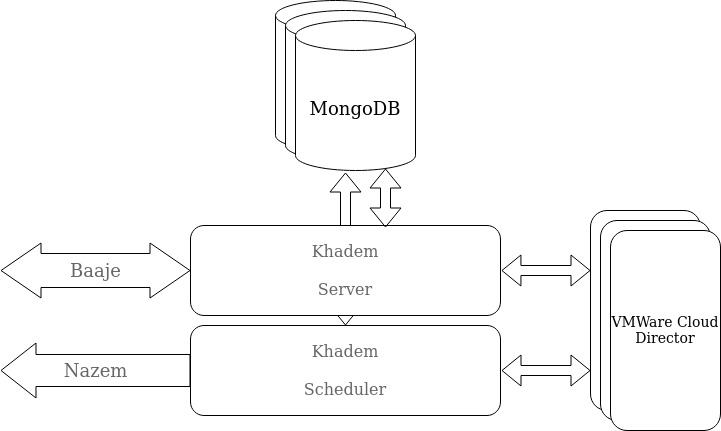
\includegraphics[scale=0.5]{figures/30bird-khadem.jpeg}
	\caption{عملکرد سرویس خادم}
	\label{fig:30bird-khadem}
\end{figure}

برنامه \textbf{زمان‌بند} در پس‌زمینه به صورت مستقل اجرا شده و در فواصل زمانی مشخص وضعیت منابع تعریف شده داخل \lr{Cloud Director} را رصد کرده و گزارش وضعیت را به سرویس ناظم جهت رسیدگی به امور مالی و نظارتی ارسال می‌کند. یک محدودیت مهم این سرویس، تک نسخه ای بودن آن در زمان اجرا است. برای قابلیت چند نسخه‌ای بودن این برنامه، بایستی یک مکانیزم و الگوریتم هماهنگی میان عناصر درحال اجرا پیاده‌سازی کنیم که منابع سیستم در هر لحظه تنها \textbf{توسط فقط یک نسخه} رصد و گزارش شود. پیاده‌سازی این موضوع با کمک امکانات کوبرنتیز امکان پذیر است ولی بخاطر پیچیدگی‌هایی که این پیاده‌سازی به همراه دارد در این پروژه از این‌کار صرف نظر شده‌است.

برنامه خدمت‌گزار در پس‌زمینه اجرا می‌شود و منتظر دستورات از سمت باجه می‌شود. پس از رسیدن دستورات، بسته به نوع دستور، توابع و پیاده‌سازی‌های موجود در بسته \lr{vcloud} در برنامه اجرا می‌شود. با این کار، دستورات قابل فهم توسط \lr{cloud director} ارسال شده و نتیجه به صورت برخط و یا غیر برخط به کاربر گزارش می‌شود.


\section{‌دروازه‌ی ورود رابط}
پیاده‌سازی ‌دروازه‌ی ورود رابط در این سامانه با استفاده از ابزار قدرتمند و پایدار \lr{nginx} صورت گرفته. \lr{nginx} یک خدمت‌گزار وب نوشته شده با زبان \lr{C} است که توانایی مدیریت تعداد بسیار زیادی از درخواست‌ها در لحظه را دارد. برای استفاده از این ‌دروازه‌ی ورود باید قوانین مربوط به مسیریابی را در فرمت مخصوص بنویسیم. از آنجایی که مقیاس کردن این گزینه به صورت افقی سخت انجام می‌شود (باید قوانین مربوط به \lr{DNS} و کاربران را تغییر دهیم.) بایستی منابع و ظرفیت‌های این برنامه‌ را زیاد‌تر از سایر قسمت‌های دیگر در نظر بگیریم.

\section{خطایابی}
عملکرد مورد انتظار رابط‌های برنامه‌نویسی برنامه در فایل‌های \lr{Open API Specification} نوشته‌شده، می‌توان این فایل‌ها را با استفاده از ابزار \lr{Swagger} بررسی کرد. در صورتی که سامانه نتیجه‌ای غیر از نتیجه انتظار برگرداند. خطایابی با استفاده از کد وضعیت برگردانده شده به همراه پیام\LTRfootnote{Message} پاسخ می‌تواند انجام شود. در صورت نیاز به اطلاعات بیشتر، برنامه‌ها خطا‌های رخ‌داده را داخل \lr{Std Error} محیط اجرایی چاپ می‌کنند. در صورت اجرا در قالب بسته‌های داکر، چک کردن این خطا‌ها می‌تواند با دستور \lr{docker logs} انجام شود. با توجه به سطوح مختلف اطلاع رسانی خطا، تنظیمات چاپ رخداد‌ها را می‌شود داخل فایل \lr{config} تغییر داد. درجات مختلف چاپ جزئیات در لیست زیر نوشته شده‌است. در این لیست اولین عضو به معنی کمترین جزئیات و آخرین عضو به معنی بیشترین جزئیات است.

\begin{enumerate}
	\item \lr{panic}
	\item \lr{fatal}
	\item \lr{error}
	\item \lr{warning}
	\item \lr{info}
	\item \lr{debug}
\end{enumerate}


\section{نتیجه گیری}
در این فصل به تشریح قسمت‌های مختلف برنامه و جزئیات پیاده‌سازی آن‌ها پرداخته شد. سامانه ما از چهار میکروسرویس که هریک وظیفه مخصوص به خود را دارد تشکیل شد. این میکروسرویس‌ها که در قالب بسته‌های داکر اجرا شدند با رابط‌های \lr{REST} به یکدیگر متصل هستند. همه این میکروسرویس‌ها در پشت یک ‌دروازه‌ی ورود قرار گرفته و راه ارتباطی با شبکه خصوصی سامانه تنها این ‌دروازه‌ی ورود است. اولین میکروسرویس درگیر با درخواست‌های کاربران، \textbf{قفل} هست که وظیفه احراز هویت تمامی درخواست‌های ورودی به ‌دروازه‌ی ورود را دارد. میکروسرویس بعدی، \textbf{باجه} است که تمامی عملیات کاربران در آن تعریف شد. این میکروسرویس برای صحت سنجی درخواست‌های کاربران با میکروسرویس \textbf{ناظم} در ارتباط است و برای انجام این درخواست‌ها با میکروسرویس \textbf{خادم} ارتباط برقرار می‌کند.


\chapter{بررسی و ارزیابی}
در این فصل به ارزیابی‌ها و بررسی‌های انجام شده بر روی پروژه پرداخته خواهد شد.

\section{تست‌های واحد}
تست واحد\LTRfootnote{Unit Test} یکی از مهم‌ترین بخش‌های ارزیابی یک برنامه است. این مدل از ارزیابی به بررسی عملکرد یک واحد از برنامه می‌پردازد. یک واحد به معنی کوچک‌ترین بخش منزوی از یک برنامه ‌است که به صورت مستقل عمل می‌کند و ورودی و خروجی مشخصی دارد. این واحد می‌تواند بخشی از یک تابع، کل تابع و یا مجموعه‌ای از توابع باشد. از مزایای تست واحد، می‌توان به صحت سنجی عملکرد واحد‌ها نسبت به ورودی‌های مختلف اشاره کرد که کمک بسیار شایانی به اجرا‌های موفق می‌کند و ریسک عملکردهای دور از انتظار را بسیار کاهش می‌دهد. 

در زبان برنامه‌نویسی \lr{Go}، این ارزیابی‌ها در سطح بسته انجام می‌شوند. فایل‌های تست، با پسوند \texttt{\_test.go} در نام فایل مشخص شده و توسط دستور \lr{go test} اجرا می‌شود. در این پروژه، ما ارزیابی‌ها را برای واحدهای مختلفی از جمله توابع رسیدگی کننده به درخواست‌ها و یا مدل‌های تعامل با پابگاه داده انجام داده ایم. این ارزیابی‌ها با اجرا کردن توابع با انواع مختلف ورودی، خروجی تابع را با خروجی مورد انتظار مقایسه می‌کنند و در صورت وجود تفاوت ارزیابی را با وضعیت خطا تمام می‌کنند. با گسترده کردن ورودی‌های ارزیابی و تقلید\LTRfootnote{Mock} کردن نیازمندی‌ها، می‌توانیم از صحت عملکرد توابع در سناریو‌های مختلف اطمینان حاصل کنیم. همچنین با استفاده از ابزار‌های مختلفی که زبان \lr{Go} برای این هدف در اختیار توسعه دهندگان قرار داده، همانند ابزار \lr{Coverage} می‌توانیم درصد پوشش تست، یعنی تعداد خط‌های کد که این تست آن‌ها را مورد ارزیابی قرار داده پیدا کنیم و مطمین شویم که کل واحد مورد ارزیابی قرار گرفته است.

% اینجا باید اسکرین شات از یونیت تست بذاریم

\section{تست‌های ادغام}
تست ادغام\LTRfootnote{Integration Test} به معنی تست کلی سامانه و ارزیابی عملکرد چندین بخش از سامانه در کنار یکدیگر است. این تست می‌تواند در داخل خود کد و همانند تست‌های واحد در قالب فایل‌های \texttt{\_test.gi} باشد. و هم می‌تواند توسط ابزار‌های خارجی و با نسخه درحال اجرای برنامه اجرا شود. یک مثال از این مدل ارزیابی، اجرای فرایند ثبت‌نام و ورود کاربر به صورت تعاملی\LTRfootnote{Interactive} با سامانه است. برای این‌کار، ابتدا با یک درخواست اقدام به ساخت حساب کاربری می‌کنیم. سپس با اطلاعات استفاده شده در مرحله قبل، اقدام به ورود و دریافت کلید ورود می‌کنیم. سپس با ارزیابی کلید ورود متوجه عملکرد این قسمت از سامانه می‌شویم.

با توجه به پیاده‌سازی رابط‌های ارتباطی وب در این پروژه با استاندارد \lr{Open API}، تمامی مقصد‌های تعریف شده. قابلیت اجرا با ورودی دلخواه توسط ابزار‌های تست \lr{API} نظیر \lr{Postman} یا \lr{K6} را دارند.

% اینجا باید یک یا چندتا تست پست من درست بکنیم و اضافه بکنیم اینجا.

\section{تست بار}
تست بار\LTRfootnote{Load Test} به دسته‌ای از تست‌ها گفته می‌شود که عملکرد سامانه و الگوی مصرف از منابع و میزان مصرف از منابع را در سناریو‌های تحت فشار شدید ارزیابی می‌کنند. معمولا این تست‌ها عملکردی ساده از سامانه که می‌تواند یک تست ادغام باشد را به صورت موازی توسط چندین کاربر اجرا می‌کنند. نتایج این تست به توسعه دهندگان این امکان را می‌دهد که نسبت حجم درخواست به منابع مصرفی و سرعت پاسخگویی برنامه را متوجه شوند و در صورت نیاز سناریو‌های مقیاس پذیری یا بهبود‌های عملکردی را طراحی کنند.

این تست‌ها در این پروژه به دو صورت انجام شده، دسته اول از تست‌ها در قالب فایل‌های \lr{Benchmark} اضافه شده. یکی از قابلیت‌های زبان برنامه‌نویسی \lr{Go}، امکان تعریف \lr{Benchmark} برای قسمت‌های مختلف برنامه است. این توابع همانند تست‌های واحد، می‌توانند واحد مشخصی از برنامه را با حجم متغیری از ورودی اجرا کنند و نتیجه را به تفکیک سرعت اجرا و منابع مصرفی برای کاربر نمایش دهند. 

% یک بنچمارک و نتیجه اش رو باید اینجا بذاریم

نوع دیگر انجام تست بار، توسط ابزار‌های خارجی اجرا می‌شود و عملکرد کلی برنامه‌را در سناریو‌های پیچیده‌تر ارزیابی می‌کند. یکی از ابزار‌های مورد استفاده در این بخش، ابزار k6 است. با نوشتن و طراحی سناریو و مشخص کردن نوع و حجم بار ورودی به سامانه، با اجرای این برنامه، می‌توانیم عملکرد سامانه را نسبت به حجم بار ورودی ارزیابی کنیم و در نهایت صحت عملکرد پاسخ‌ها را نیز دریافت کنیم.

% نمونه ای از اجرای k6 و جوابش


\section{محدودیت‌ها}
با توجه به معماری استفاده‌شده در پیاده‌سازی این سامانه، تمامی خدمت‌گزار‌های سامانه و پایگاه داده می‌توانند به صورت افقی مقیاس شوند تا پاسخگوی حجم‌های احتمالی زیاد باشند. با این وجود بخش‌هایی از سامانه محدودیت‌هایی در راستای حجم فشار کلی سامانه ایجاد می‌کنند.


اولین محدودیت سامانه، عدم امکان مقیاس کردن زمان‌بند سرویس خادم است. این زمان‌بند به صورت مستقیم با کاربران در تعامل نیست و در نتیجه حجم درخواست‌های ناگهانی بار اصلا تاثیرگذار نیست. اما بالا رفتن تعداد منابع ساخته‌شده، یا فشار زیاد شبکه، باعث اختلال در عملکرد و فشار بر این برنامه می‌شود. راه حل کمتر کردن این فشار، رزرو کردن منابع اختصاصی شبکه برای این برنامه در کنار زیاد کردن منابع محاسباتی پیش از اجرا است.

یکی دیگر از محدودیت‌های سامانه که مقیاس شدن برنامه در آن تاثیر کمی دارد، زیرساخت \lr{cloud director} است. با توجه به ساختار تک نسخه‌ای بودن آن در برنامه، تمامی نسخه‌های سرویس خادم با یک نسخه‌از \lr{cloud director} در ارتباط هستند. از آنجایی که عملیات‌های تعریف شده در این برنامه، ذاتا زمان‌بر هستند و نیازمند اجرا به صورت آسنکرون هستند. اجرای حجم زیادی از درخواست‌ها و ارسال آن‌ها به سمت \lr{cloud director} می‌تواند باعث بروز اختلال و اعمال فشار بر این سرویس شود. راه حل پیشنهادی جهت بهبود این محدودیت، تعریف سقف برای تعداد عملیات‌های در حال اجرا در سمت خادم است. این‌کار می‌تواند با قرار دادن یک صف پیام\LTRfootnote{Message Queue} بین سرویس باجه و خادم انجام شود.

\clearpage
\section{خطایابی}
عملکرد مورد انتظار رابط‌های برنامه‌نویسی برنامه در فایل‌های \lr{Open API Specification} نوشته‌شده، می‌توان این فایل‌ها را با استفاده از ابزار \lr{Swagger} بررسی کرد. در صورتی که سامانه نتیجه‌ای غیر از نتیجه انتظار برگرداند. خطایابی با استفاده از کد وضعیت برگردانده شده به همراه پیام\LTRfootnote{Message} پاسخ می‌تواند انجام شود. در صورت نیاز به اطلاعات بیشتر، برنامه‌ها خطا‌های رخ‌داده را داخل \lr{Std Error} محیط اجرایی چاپ می‌کنند. در صورت اجرا در قالب بسته‌های داکر، چک کردن این خطا‌ها می‌تواند با دستور \lr{docker logs} انجام شود. با توجه به سطوح مختلف اطلاع رسانی خطا، تنظیمات چاپ رخداد‌ها را می‌شود داخل فایل \lr{config} تغییر داد. درجات مختلف چاپ جزئیات در لیست زیر نوشته شده. در این لیست اولین عضو به معنی کمترین جزئیات و آخرین عضو به معنی بیشترین جزئیات است.

\begin{enumerate}
	\item \texttt{panic}
	\item \texttt{fatal}
	\item \texttt{error}
	\item \texttt{warning}
	\item \texttt{info}
	\item \texttt{debug}
\end{enumerate}

\chapter{جمع‌بندی، نتیجه‌گیری و پیشنهادات برای کارهای آتی}
\section{جمع‌بندی و نتیجه‌گیری}
در این پروژه، سعی کردیم که یک رابط تحت وب برای ارائه خدمات \lr{IaaS} بر بستر \lr{VMWare Cloud Director} ارائه دهیم. در ابتدا با تحقیق و پیدا کردن نیازمندی‌ها، اقدام به طراحی معماری کلی سامانه و شناسایی ابزار‌ها و نیازمندی‌ها کردیم. سپس با تحقیق در مورد این نیازمندی‌ها و مزیت‌های هر مدل از پیاده‌سازی، به یک طراحی نهایی رسیدیم. برای طراحی این پیاده‌سازی از الگو‌های رایج توسعه نرم‌افزار تحت وب استفاده کردیم و به یک سامانه با قابلیت‌های قبول رسیدیم که به واسطه ساختار قطعه‌ای، قابلیت توسعه و تکمیل کردن به راحتی‌را دارد. سپس با ارزیابی‌های چندجانبه از صحت و توان عملکردی نرم‌افزار، پیش‌بینی تقریبی از اجرای این نرم‌افزار در سناریو‌های واقعی به دست آوردیم.

\section{پیشنهادات برای کارهای آتی}
این پروژه، قابلیت تکمیل و توسعه از ابعاد مختلفی را داراست. ساختار میکروسروییسی و وابستگی اندک سرویس‌ها به یکدیگر، امکان توسعه و تغییر در میکروسرویس‌ها را به صورت جداگانه می‌دهد. در ادامه برخی پیشنهادات برای تکمیل و توسعه را به صورت جامع توضیح می‌دهیم.

\subsection{تجزیه میکروسرویس ناظم}
عملکرد سرویس ناظم در حال حاضر، دربرگیرنده تنظیمات و تصمیمات کسب‌و‌کار از جمله مصرف کاربران و امور مالی است. در صورت نیاز و ظهور نیازمندی‌های کسب‌و‌کاری بیشتر، می‌توان قسمت ثبت مصرف و تصمیمات مالی را جداکرد. 

با این‌کار می‌توان مدل‌های مختلف پرداختی را پشتیبانی کرد. این جداسازی مزیت جداشدن منطق و محدودتر شدن فعالیت‌های میکروسرویس را به دنبال دارد. منتها سربار منابع مصرفی اضافی و افزایش تعداد درخواست‌ها در شبکه را نیز اضافه می‌کند.


\subsection{ارتباطات رخداد پایه}
در حال حاضر، تمام ارتباطات سامانه به صورت سنکرون و توسط درخواست‌های \lr{HTTP} انجام می‌شود. مزیت این روش سادگی پیاده‌سازی و دنبال کردن روند اجرای‌ دستورات است. منتها با افزایش تعداد درخواست‌ها و محدودیت‌های شبکه ، این مشکل پیش می‌آید که بازیابی وضعیت سیستم از خطا دشوارتر می‌شود. برای افزایش آستانه تحمل خطا در سرویس‌ها و امکان اضافه کردن تلاش مجدد\LTRfootnote{Retry}، می‌توان ارتباط سرویس‌ها را به صورت آسنکرون و به صورت رخداد پایه انجام داد. مزیت این‌کار بالابردن در دسترس بودن سیستم\LTRfootnote{Availability} می‌شود. برای پیاده‌سازی این مورد می‌توان از ابزارهای انتقال پیام نظیر \lr{Apache Kafka} یا راه‌حل‌های سبک‌تر نظیر \lr{NATS} استفاده کرد. 

نحوه پیاده‌سازی \lr{API} در میکروسرویس‌ها، امکان تغییر مکانیزم تعامل با بیرون را بسیار ساده کرده است. فقط کافی‌است که در پکیج‌های مربوطه، توابع مربوط به دریافت و ارسال اطلاعات را فارغ از نحوه پیاده‌سازی معرفی کنید. لایه‌های زیرین سرویس فقط نیازمند توابعی برای دریافت و ارسال اطلاعات هستند و وابستگی‌ای به نحوه دریافت و ارسال این اطلاعات ندارند.

معماری جدید سامانه در این حالت در شکل\ref{fig:30bird-cmq} مشخص شده است.

\begin{figure}
	\centering
	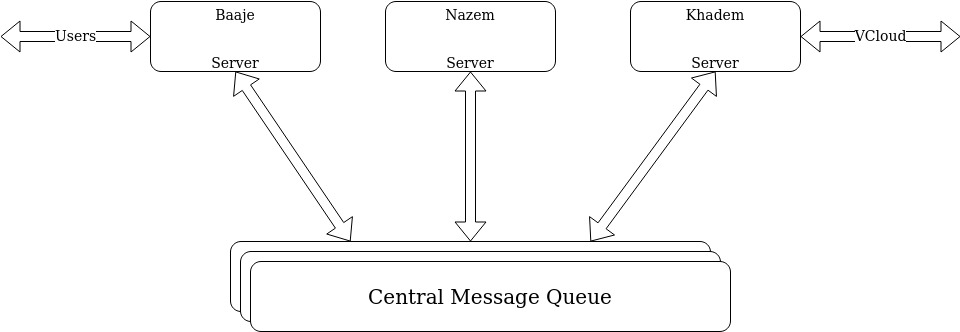
\includegraphics[scale=0.45]{figures/30bird-cmq.jpg}
	\caption{معماری سامانه در حالت آسنکرون}
	\label{fig:30bird-cmq}
\end{figure}


\subsection{نظارت و گزارش رخداد‌ها}
جهت بهبود وضعیت نظارت بر سامانه، می‌توان از داشبورد‌های گرافیکی ابزار گرافانا\LTRfootnote{Grafana} استفاده کرد. فقط کافیست که از اطلاعات متریک‌های سرور برای نمایش اطلاعات در قالب این داشبورد‌ها استفاده‌کرد.

مزیت دیگر استفاده از این ابزار، امکان تعریف هشدار\LTRfootnote{Alert} برای وضعیت‌های خاص و ناخواسته است. استفاده از این الگو، از روند‌های رایج در فرهنگ \lr{SRE}\LTRfootnote{Software Reliability Engineer} است. پیروی از این فرهنگ، بازیابی از فاجعه‌ها و ایرادات را بسیار سریع‌تر و آسان‌تر می‌کند.

اضافه کردن \lr{Telemetry} بسیار به درک و نظارت عملکرد میکروسرویس‌ها کمک می‌کند. ابزار پیشنهادی برای پیاده‌سازی این قابلیت، \lr{Jaeger} و کتاب‌خانه‌های \lr{OpenTelemetry} است.

\subsection{پشتیبانی از افزونه‌های \lr{VMWare Cloud Director}}
برخی از قابلیت‌های ابزار \lr{Cloud Director} در قالب افزونه‌ها ارائه شده که به صورت پیش‌فرض فعال نیستند و نیازمند تغییراتی در تنظیمات هستند. با فعال سازی این افزونه‌ها می‌توان از امکانات بیشتری از این سرویس استفاده کرد. یکی از مثال‌های این افزونه‌ها، افزونه نظارت (\lr{Monitoring}) است که نیازمند راه‌اندازی یک پایگاه \lr{Cassandra} است. با تنظیم کردن و اضافه کردن این افزونه، امکان دریافت جزئیات مصرف منابع و گزارش گیری از آنها را مستقیما از سمت \lr{Cloud Director} پیدا می‌کنیم.

البته پیاده‌سازی این این امکانات در سمت سرویس خادم با چالش‌هایی همراه است. چرا که این جزئیات در بسته توسعه نرم‌افزار پیش‌فرض تعبیه نشده و نیازمند تعامل مستقیم و خام برنامه با رابط برنامه‌نویسی \lr{vCloud} است. البته این امر می‌تواند به سادگی و با تبدیل دستورات برنامه رابط کاربری تحت وب به دستورات \lr{cURL} و سپس تبدیل دستورات \lr{cURL} به درخواست‌های \lr{HTTP} در زبان \lr{Go} توسط برنامه \lr{Postman} انجام شود. توسعه‌دهنده کافی است درخواست‌های ساخته‌شده را به قالب توابع موجود \texttt{VCloudManager} در بسته \texttt{vcloud} در برنامه تبدیل کند.

%--------------------------------------------------------------------------appendix( مراجع و پیوست ها)
\chapterfont{\vspace*{-2em}\centering\LARGE}%


\appendix
\bibliographystyle{plain-fa}
\begingroup
\raggedright
\bibliography{references}
\endgroup

\chapter*{‌پیوست}
\markboth{پیوست}{}

% براي شماره‌گذاري روابط، جداول و اشكال موجود در پيوست‌ از ساختار متفاوتي نسبت به متن اصلي استفاده مي‌شود كه در زير به‌عنوان نمونه نمايش داده شده‌است. 

\section*{کد‌ها و پیوست‌ها}
تمامی‌ کد‌ها و پیوست‌های پروژه نظیر ساختار پایگاه‌داده، نیازمندی‌های اجرا و فایل‌های قابل اجرا در مخزن زیر در دسترس است.
\begin{latin}
	\href{https://github.com/smf8/30bird}{\texttt{https://github.com/smf8/30bird}}
\end{latin}

\section*{نمودار‌های رابطه-موجودیت}

\begin{figure}
	\centering
	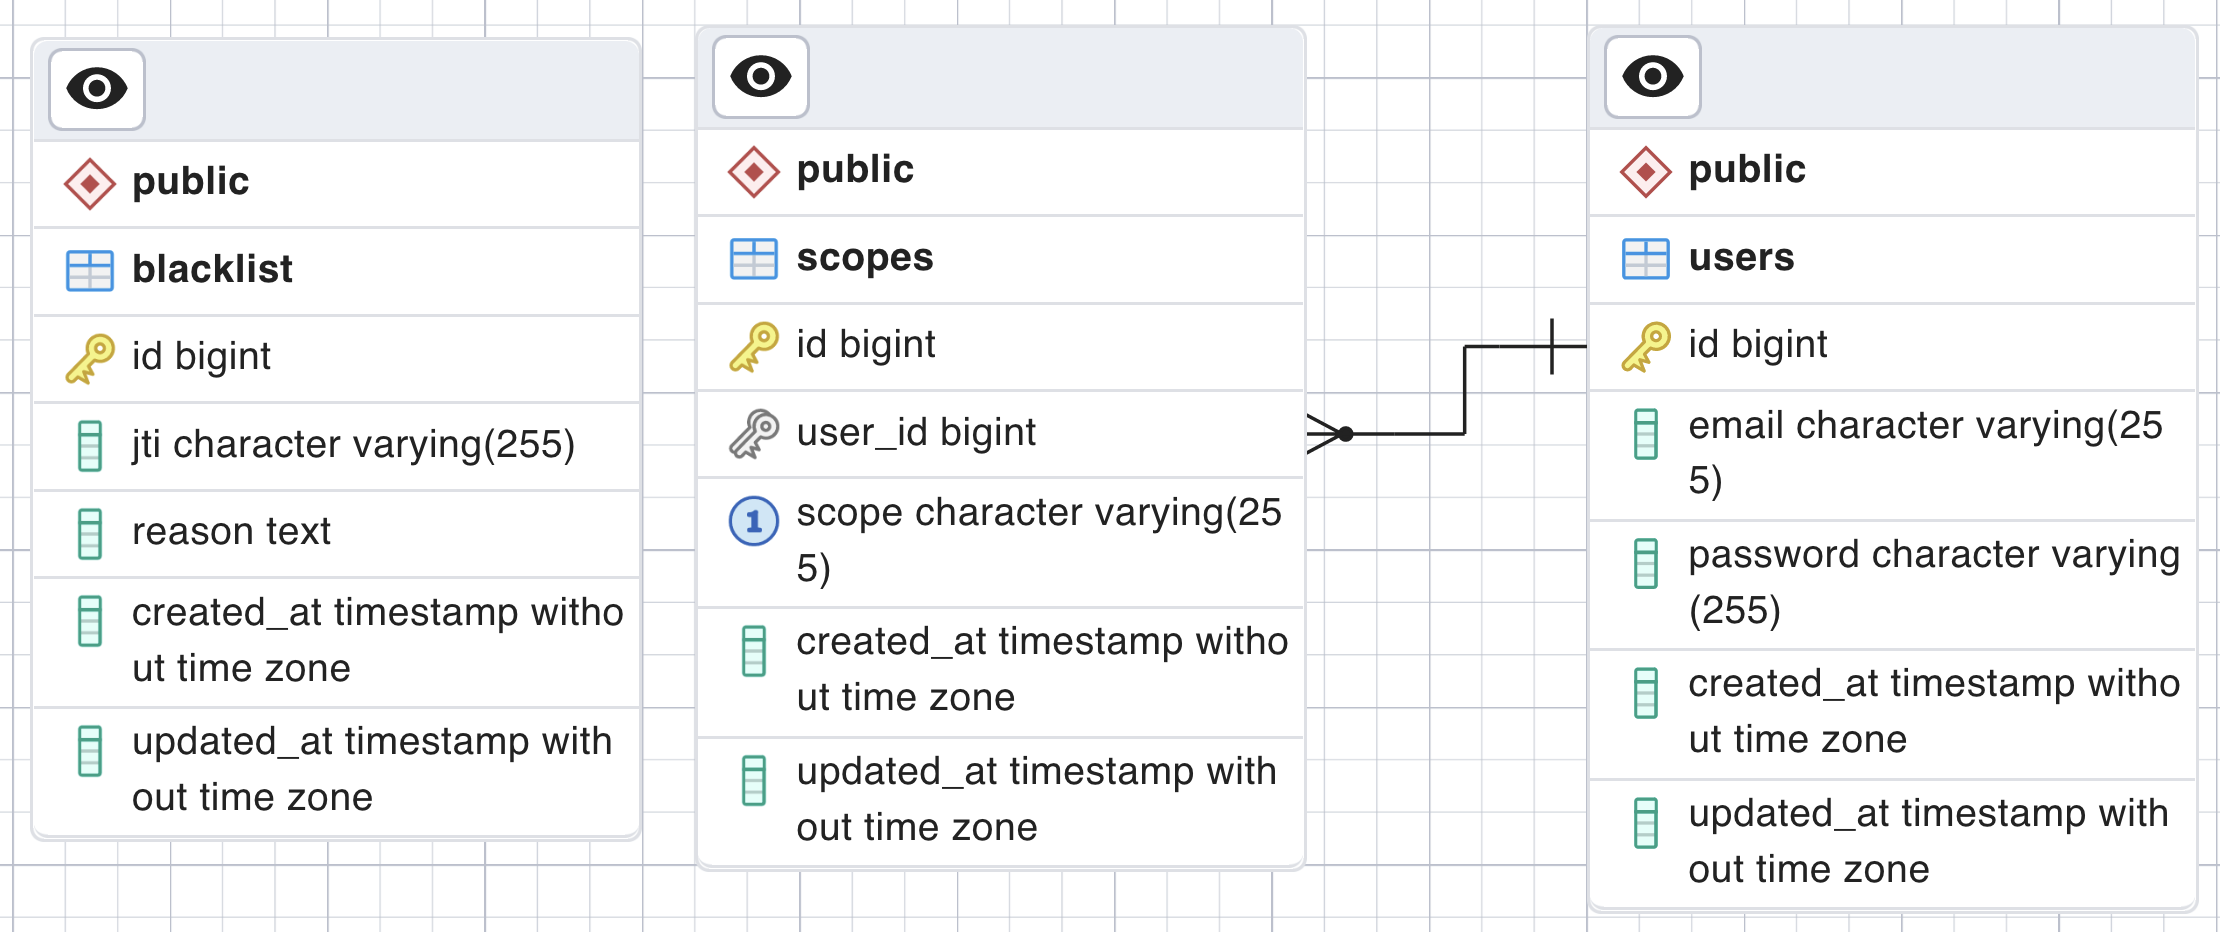
\includegraphics[width=0.9\linewidth]{figures/erd-ghofl}
	\caption{ساختار موجودیت‌ها و رابطه‌ها در پایگاه داده قفل}
	\label{fig:erd-ghofl}
\end{figure}

\begin{figure}
	\centering
	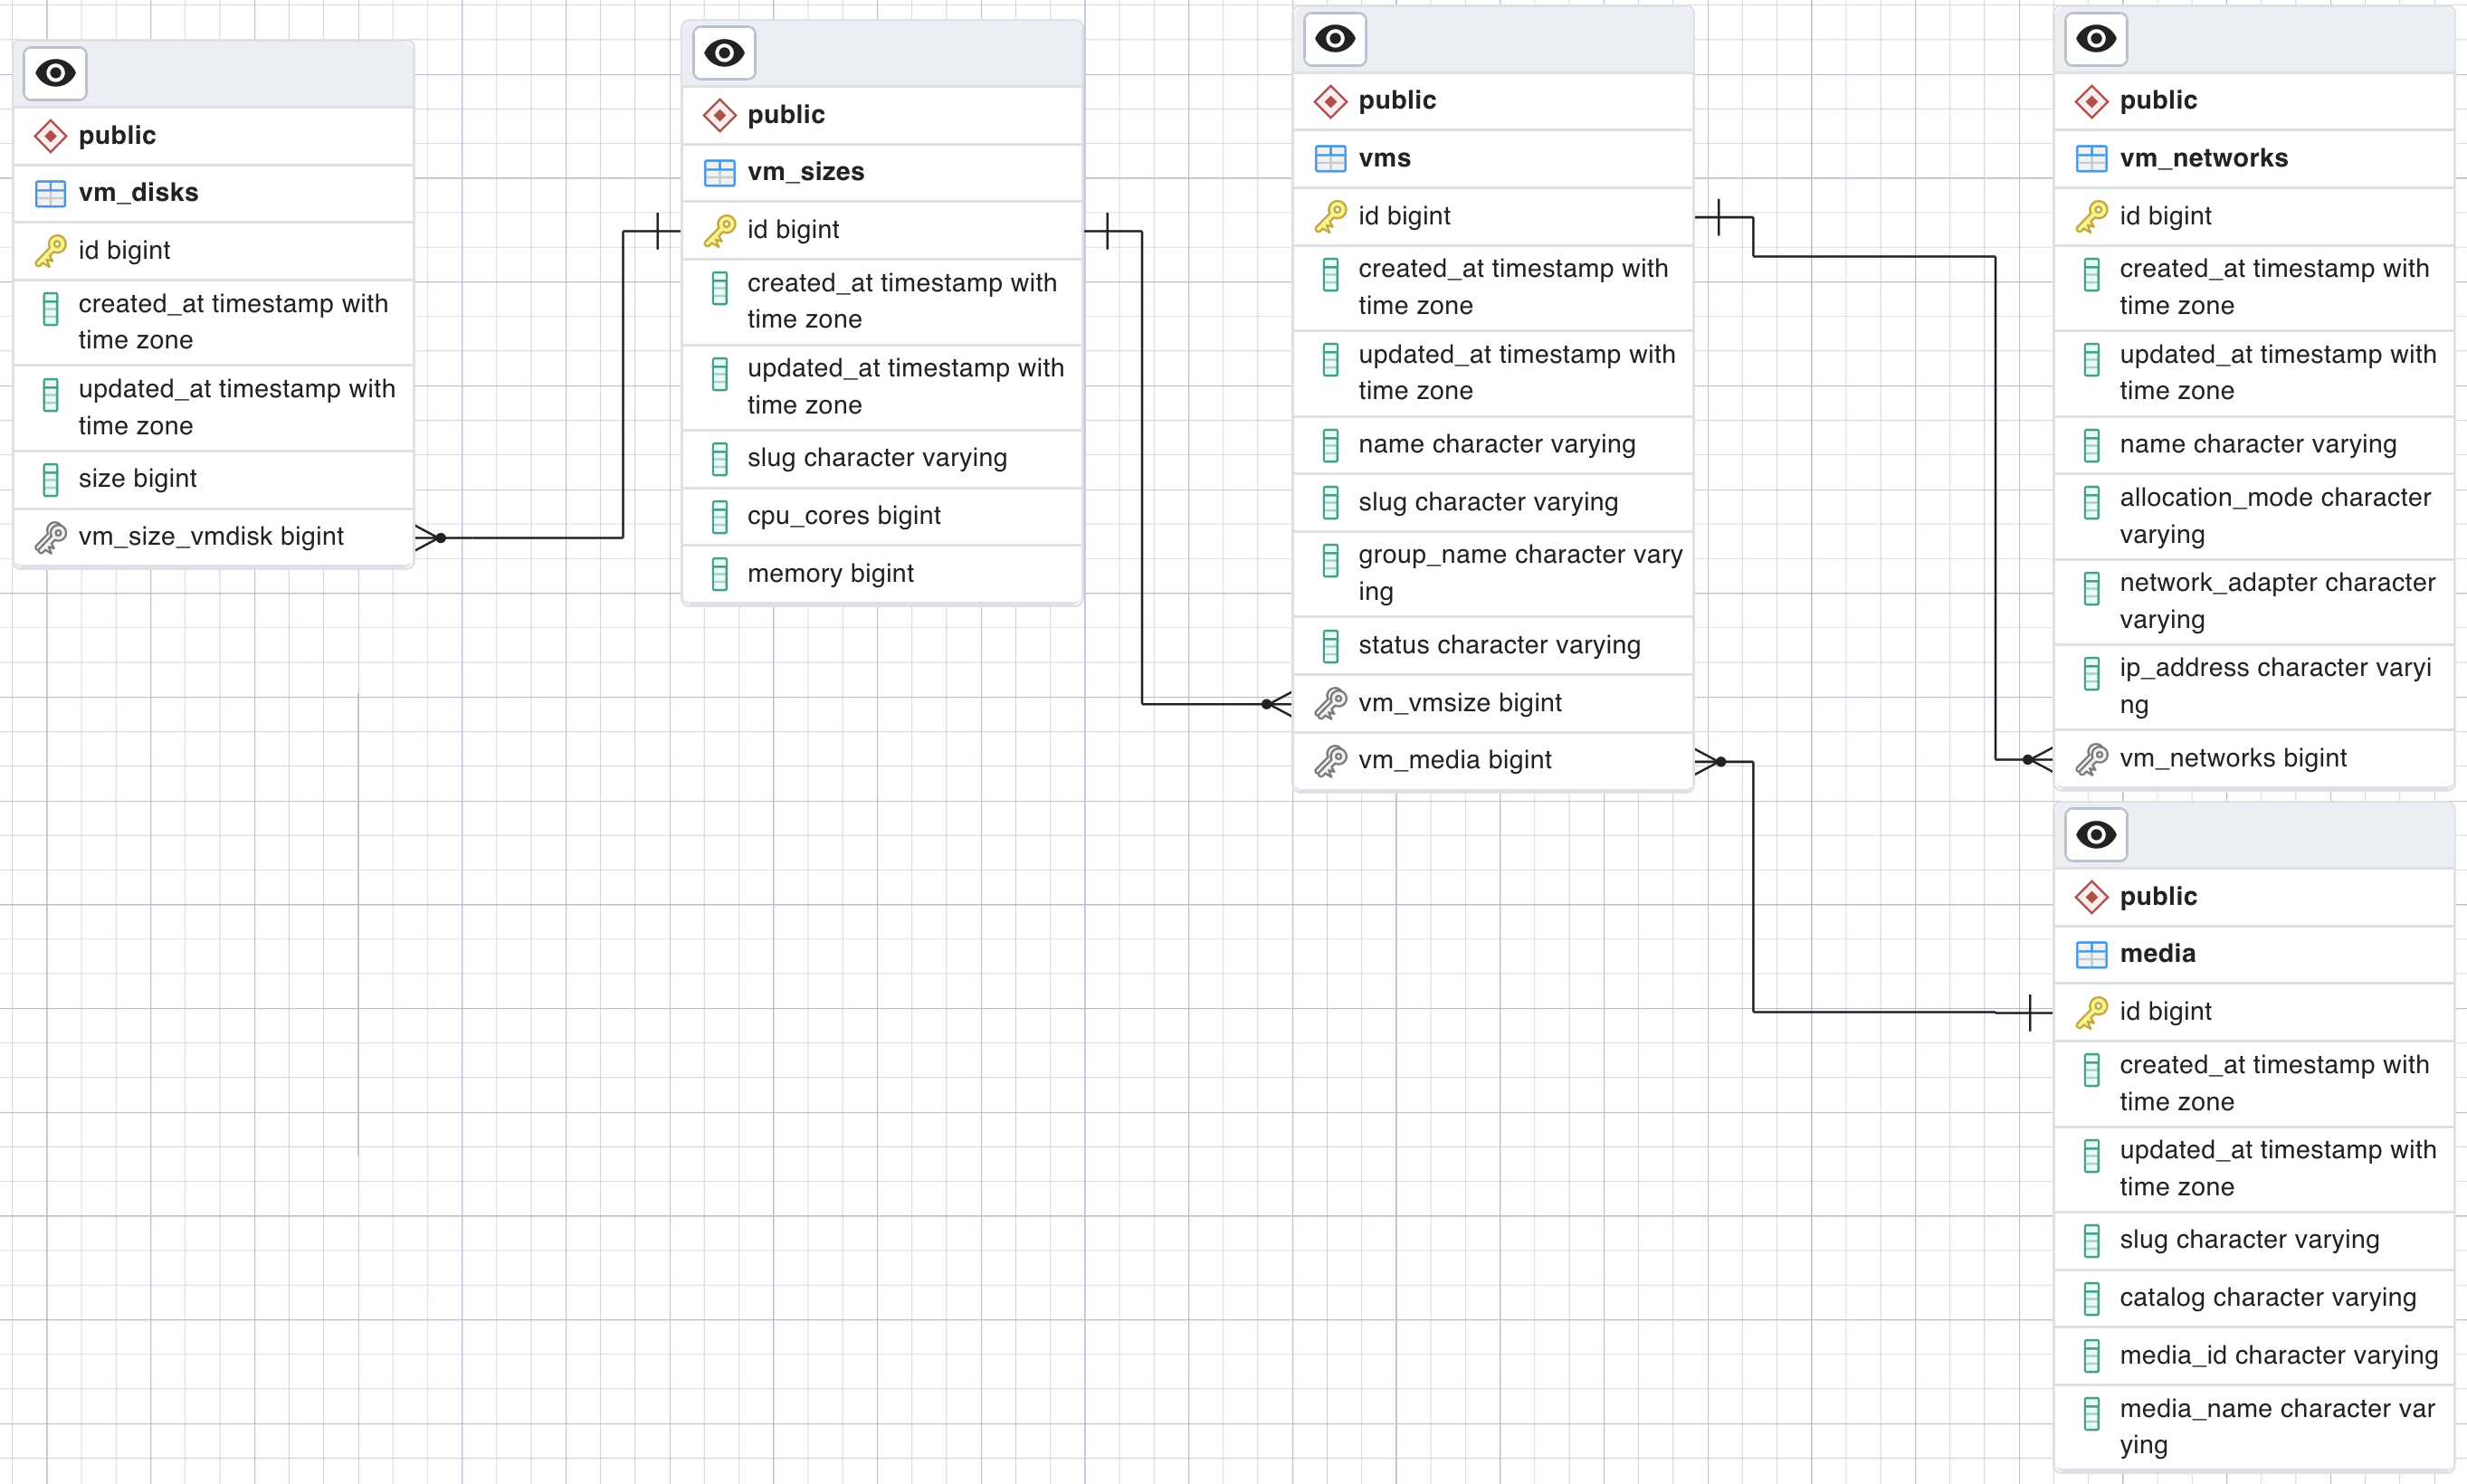
\includegraphics[width=1\linewidth]{figures/erd-baaje}
	\caption{ساختار موجودیت‌ها و رابطه‌ها در پایگاه داده باجه}
	\label{fig:erd-baaje}
\end{figure}

\begin{figure}
	\centering
	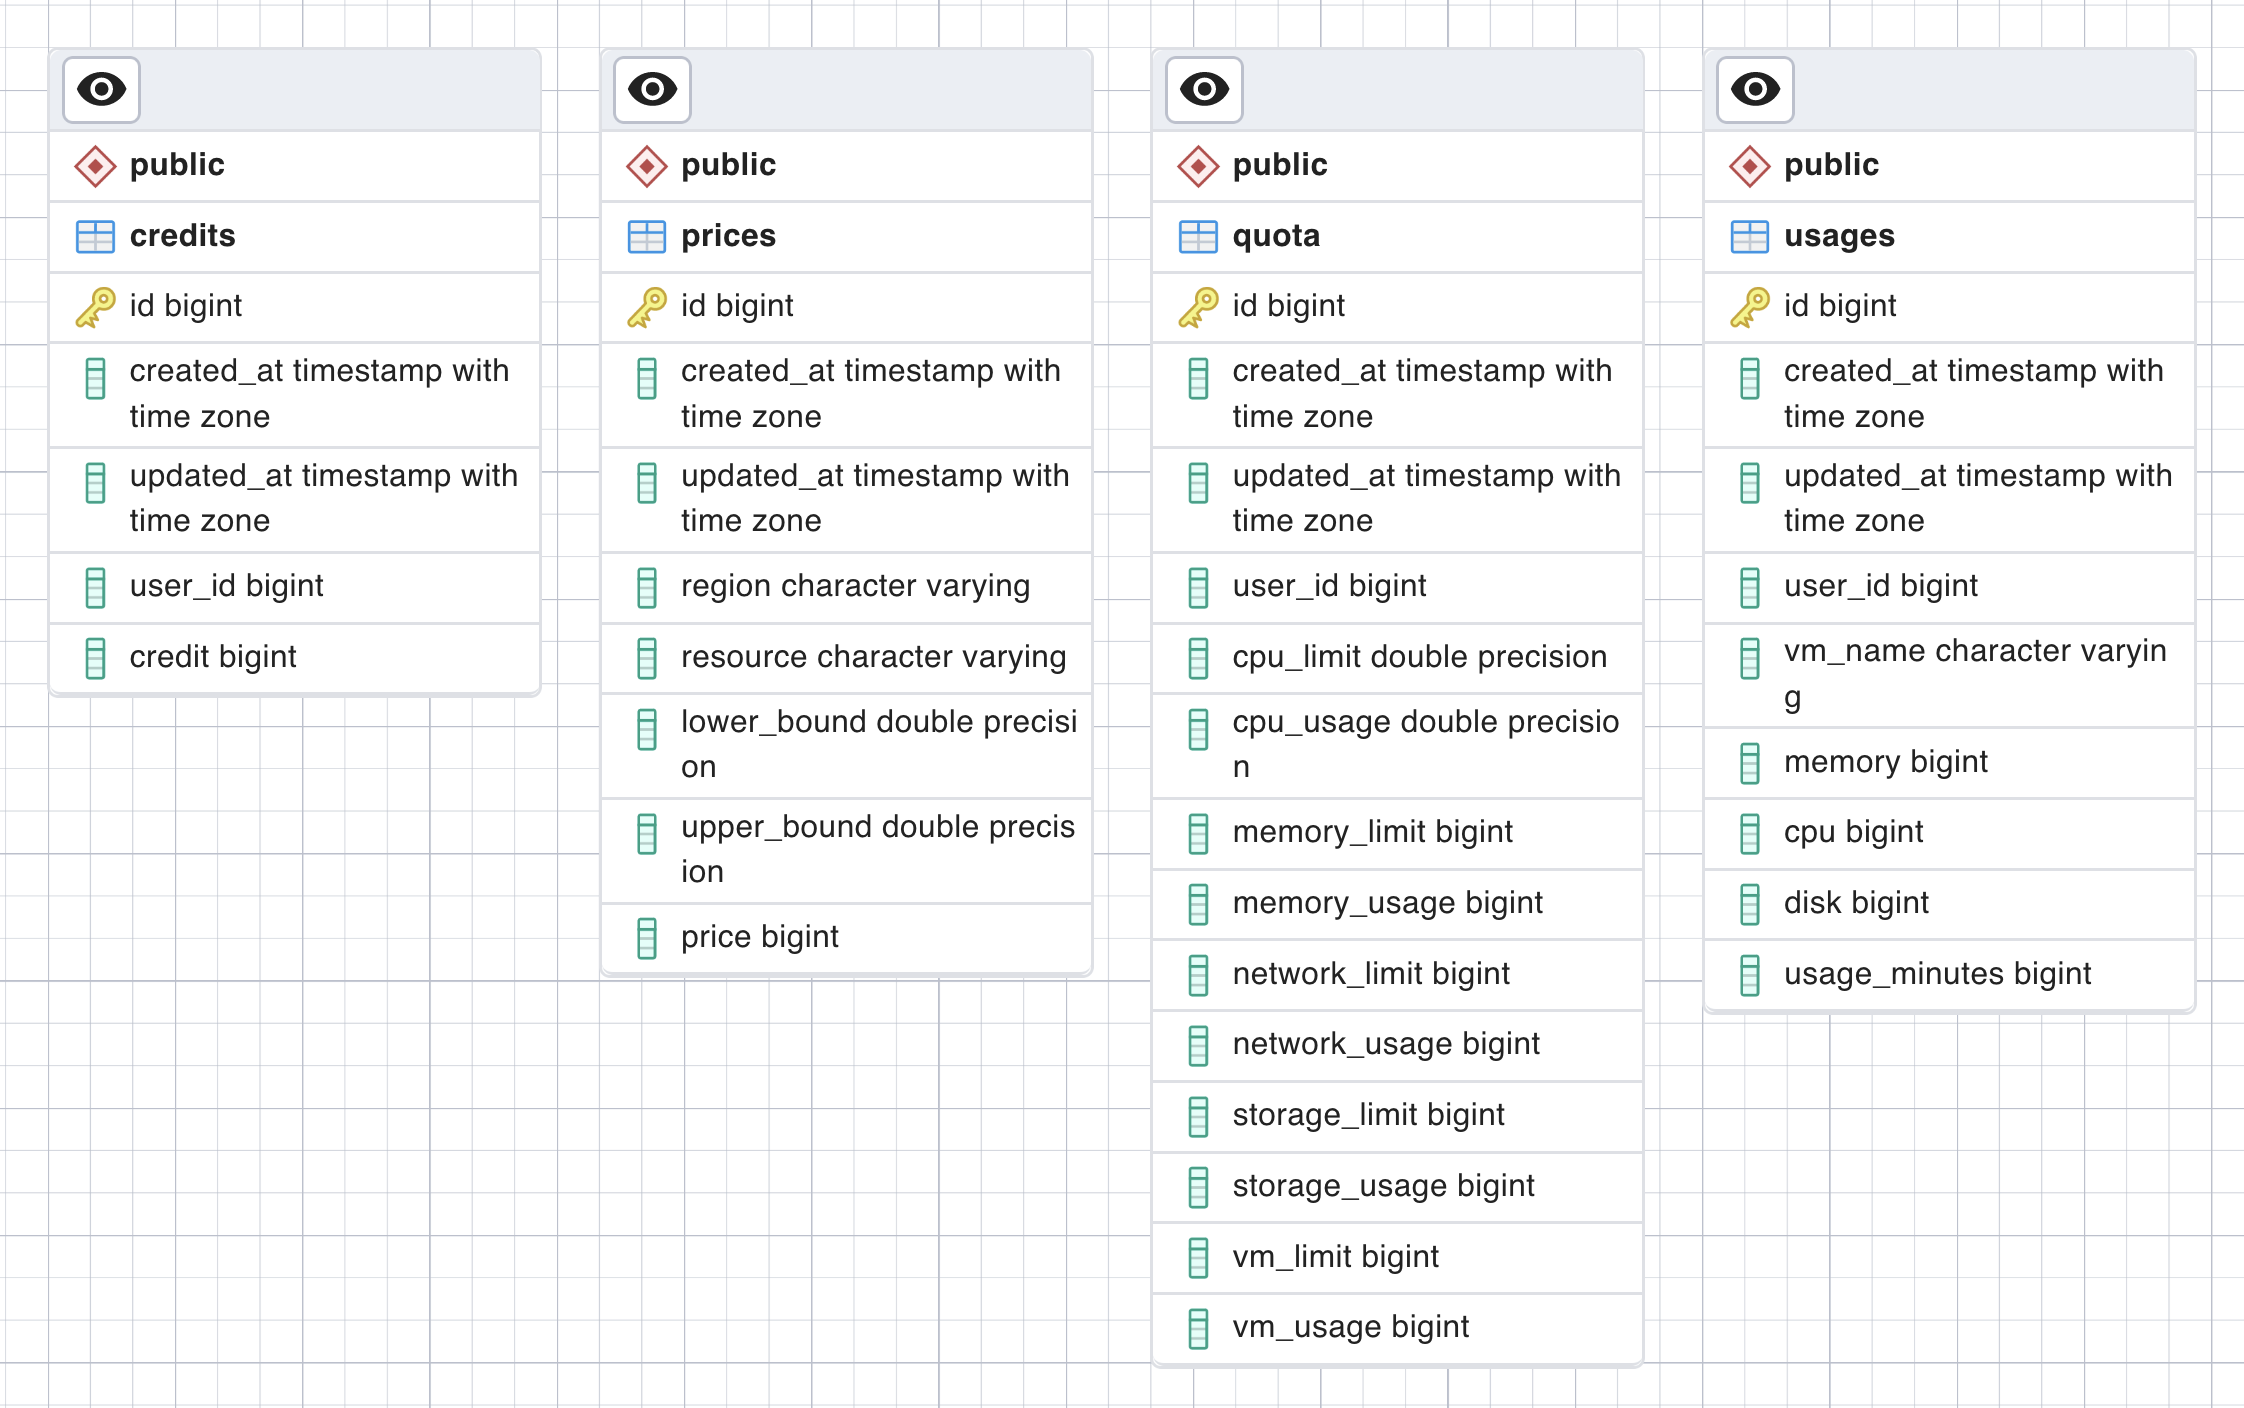
\includegraphics[width=\linewidth]{figures/erd-nazem}
	\caption{ساختار موجودیت‌ها در پایگاه داده ناظم}
	\label{fig:erd-nazem}
\end{figure}


%--------------------------------------------------------------------------dictionary(واژه نامه ها)
%اگر مایل به داشتن صفحه واژه‌نامه نیستید، خط زیر را غیر فعال کنید.
%\parindent=0pt
%%
\chapter*{واژه‌نامه‌ی فارسی به انگلیسی}
\pagestyle{style9}

\addcontentsline{toc}{chapter}{واژه‌نامه‌ی فارسی به انگلیسی}
%%%%%%
\begin{multicols*}{2}

{\bf آ}
\vspace*{3mm}


\farsiTOenglish{اسکالر}{Scalar}


\vspace*{3mm}
{\bf ب}
\vspace*{3mm}

\farsiTOenglish{بالابر}{Lift}


\vspace*{3mm}
{\bf پ}
%%\vspace*{3mm}

\farsiTOenglish{پایا}{Invariant}



\vspace*{3mm}
{\bf ت}
%%\vspace*{3mm}

\farsiTOenglish{ تناظر }{Correspondence}


\vspace*{3mm}
{\bf ث}
%%\vspace*{3mm}

\farsiTOenglish{ثابت‌ساز}{Stabilizer}

\vspace*{3mm}
{\bf ج}
%%\vspace*{3mm}

\farsiTOenglish{جایگشت}{Permutation}



\vspace*{3mm}
{\bf چ}
%%\vspace*{3mm}


\farsiTOenglish{چند جمله‌ای }{Polynomial}

\vspace*{3mm}
{\bf ح}
%%\vspace*{3mm}

\farsiTOenglish{حاصل‌ضرب دکارتی}{Cartesian product}


\vspace*{3mm}
{\bf خ}
%%\vspace*{3mm}

\farsiTOenglish{خودریختی}{Automorphism}

\vspace*{3mm}
{\bf د}
%%\vspace*{3mm}

\farsiTOenglish{درجه}{Degree}


\vspace*{3mm}
{\bf ر}
%%\vspace*{3mm}


\farsiTOenglish{ریزپردازنده}{microprocessor}


\vspace*{3mm}
{\bf ز}
%%\vspace*{3mm}


\farsiTOenglish{زیرمدول}{Submodule}


\vspace*{3mm}
{\bf س}
%%\vspace*{3mm}

\farsiTOenglish{سرشت}{Character}


\vspace*{3mm}
{\bf ص}
%%\vspace*{3mm}

\farsiTOenglish{صادقانه}{Faithful}

\vspace*{3mm}
{\bf ض}
%%\vspace*{3mm}

\farsiTOenglish{ضرب داخلی}{Inner product}

\vspace*{3mm}
{\bf ط}
%%\vspace*{3mm}


\farsiTOenglish{طوقه}{Loop}


\vspace*{3mm}
{\bf ظ}
%%\vspace*{3mm}


\farsiTOenglish{ظرفیت}{Valency}
 
\vspace*{3mm}
{\bf ع}
%%\vspace*{3mm}


\farsiTOenglish{عدم مجاورت}{Nonadjacency}



\vspace*{3mm}
{\bf ف}
%%\vspace*{3mm}

\farsiTOenglish{فضای برداری}{Vector space}



\vspace*{3mm}
{\bf ک}
%%\vspace*{3mm}

\farsiTOenglish{کاملاً تحویل‌پذیر}{Complete reducibility}


\vspace*{3mm}
{\bf گ}
%%\vspace*{3mm}


\farsiTOenglish{گراف}{Graph}



\vspace*{3mm}
{\bf م}
%%\vspace*{3mm}

\farsiTOenglish{ماتریس جایگشتی}{Permutation matrix }


\vspace*{3mm}
{\bf ن}
%%\vspace*{3mm}

\farsiTOenglish{ناهمبند}{Disconnected}


\vspace*{3mm}
{\bf و}
%%\vspace*{3mm}

\farsiTOenglish{وارون‌پذیر}{Invertible}


\vspace*{3mm}
{\bf ه}
%%\vspace*{3mm}

\farsiTOenglish{همبند}{Connected}



\vspace*{3mm}
{\bf ی}
%%\vspace*{3mm}

\farsiTOenglish{یال}{Edge}




\end{multicols*}%
%%%%%%%
\chapter*{ واژه‌نامه‌ی انگلیسی به فارسی}
\pagestyle{style9}
\lhead{\thepage}\rhead{واژه‌نامه‌ی انگلیسی به فارسی}
\addcontentsline{toc}{chapter}{واژه‌نامه‌ی انگلیسی به فارسی}

\LTRmulticolcolumns
\begin{multicols}{2}
{\hfill\bf  \lr{A}}
%%\vspace*{1.5mm}

\englishTOfarsi{Automorphism}{خودریختی}

\vspace*{3mm}
{\hfill\bf   \lr{B}}
%%\vspace*{1.5mm}

\englishTOfarsi{Bijection}{دوسویی}

\vspace*{3mm}
{\hfill\bf   \lr{C}}
%%\vspace*{1.5mm}

\englishTOfarsi{Cycle group}{گروه دوری}

\vspace*{3mm}
{\hfill\bf   \lr{D}}
%%\vspace*{1.5mm}

\englishTOfarsi{Degree}{درجه}

\vspace*{3mm}
{\hfill\bf   \lr{E}}
%%\vspace*{1.5mm}

\englishTOfarsi{Edge}{یال}

\vspace*{3mm}
{\hfill\bf   \lr{F}}
%%\vspace*{1.5mm}

\englishTOfarsi{Function}{تابع}

\vspace*{3mm}
{\hfill\bf   \lr{G}}
%%\vspace*{1.5mm}

\englishTOfarsi{Group}{گروه}

\vspace*{3mm}
{\hfill\bf   \lr{H}}
%%\vspace*{1.5mm}

\englishTOfarsi{Homomorphism}{همریختی}

\vspace*{3mm}
{\hfill\bf   \lr{I}}
%%\vspace*{1.5mm}

\englishTOfarsi{Invariant}{پایا}

\vspace*{3mm}
{\hfill\bf   \lr{L}}
%%\vspace*{1.5mm}

\englishTOfarsi{Lift}{بالابر}

\vspace*{3mm}
{\hfill\bf   \lr{M}}
%%\vspace*{1.5mm}

\englishTOfarsi{Module}{مدول}

\vspace*{3mm}
{\hfill\bf   \lr{N}}
%%\vspace*{1.5mm}

\englishTOfarsi{Natural map}{نگاشت طبیعی}

\vspace*{3mm}
{\hfill\bf   \lr{O}}
%%\vspace*{1.5mm}

\englishTOfarsi{One to One}{یک به یک}

\vspace*{3mm}
{\hfill\bf   \lr{P}}
%%\vspace*{1.5mm}

\englishTOfarsi{Permutation group}{گروه جایگشتی}

\vspace*{3mm}
{\hfill\bf   \lr{Q}}
%%\vspace*{1.5mm}

\englishTOfarsi{Quotient graph}{گراف خارج‌قسمتی}

 \vspace*{3mm}
{\hfill\bf   \lr{R}}
%%\vspace*{1.5mm}

\englishTOfarsi{Reducible}{تحویل پذیر}

\vspace*{3mm}
{\hfill\bf   \lr{S}}
%%\vspace*{1.5mm}

\englishTOfarsi{Sequence}{دنباله}

 \vspace*{3mm}
{\hfill\bf   \lr{T}}
%%\vspace*{1.5mm}

\englishTOfarsi{Trivial character}{سرشت بدیهی}

\vspace*{3mm}
{\hfill\bf   \lr{U}}
%%\vspace*{1.5mm}

\englishTOfarsi{Unique}{منحصربفرد}

\vspace*{3mm}
{\hfill\bf   \lr{V}}
%%\vspace*{1.5mm}

\englishTOfarsi{Vector space}{فضای برداری}
\end{multicols}
%--------------------------------------------------------------------------index(نمایه)
%اگر مایل به داشتن صفحه نمایه نیستید، خط زیر را غیر فعال کنید.
%\pagestyle{style7}
%\printindex
%\pagestyle{style7}
%%کلمات کلیدی انگلیسی
\latinkeywords{Write a 3 to 5 KeyWords is essential. Example: AUT, M.Sc., Ph. D,..}
%چکیده انگلیسی

\en-abstract{
This page is accurate translation from Persian abstract into English.
}
%%%%%%%%%%%%%%%%%%%%% کدهای زیر را تغییر ندهید.

\newpage
\thispagestyle{empty}
\begin{latin}
\section*{\LARGE\centering Abstract}

\een-abstract

\vspace*{.5cm}
{\large\textbf{Key Words:}}\par
\vspace*{.5cm}
\elatinkeywords
\end{latin}
% در این فایل، عنوان پایان‌نامه، مشخصات خود و چکیده پایان‌نامه را به انگلیسی، وارد کنید.
%%%%%%%%%%%%%%%%%%%%%%%%%%%%%%%%%%%%
\baselineskip=.6cm
\begin{latin}
\latinfaculty{Department of Computer Engineering}

\latintitle{VMWare VCloud IaaS REST Interface}

\firstlatinsupervisor{Dr. Mahmoud Momtazpour}

%\secondlatinsupervisor{Second Supervisor}

% \firstlatinadvisor{Dr. Mehdi Homayounpour}

%\secondlatinadvisor{Second Advisor}

\latinname{Seyed Mohammad}

\latinsurname{Fatemi}

\latinthesisdate{March 2023}

\latinvtitle
\end{latin}

\end{document}